\documentclass{article}
\usepackage[a4paper,top=3cm,bottom=3cm,left=3cm,right=3cm]{geometry}
\usepackage[utf8]{inputenc}
\usepackage[italian]{babel}
\usepackage{tabto}
\usepackage{graphicx}

\title{Gestione di un azienda vinicola}\date{}
\author{Marica Pasquali - matricola 0000802302}

\begin{document}
\maketitle  

\newpage
\tableofcontents
\newpage
\section{Analisi}
\subsection{Raccolta dei Requisiti}
Le seguente descrizione riporta in linguaggio naturale i requisiti per la gestione di un'azienda vinicola.\\
\newline
\newline
\textit{L'azienda assume, in una certa data, i vari dipendenti che svolgeranno il lavoro sul campo. Per ogni proprietario o socio dell'azienda, si vuole memorizzare nome, cognome, data di nascita, indirizzo, telefono.
Il proprietario può gestire : le varie operazioni di inserimento, modifica e di ricerca di ogni operazione che compie ogni dipendente e le vendite. Egli può accedere al software con credenziali di amministratore.
Per ogni dipendente si vuole memorizzare il numero identificativo, il nome, il cognome, la data di nascita, l'indirizzo (via, numero civico e città) e il numero di telefono.
Nel qual caso sia un dipendente part – time si vogliono memorizzare le ore di lavoro effettuate in un determinato giorno e le ore totali compiute nel corso della loro assunzione, invece nel caso di un dipendente a tempo indeterminato è inserito lo stipendio mensile.
Il dipendente part – time può partecipare a tutte le fasi della produzione del vino, ma non alla vendita.
Ogni dipendente avrà accesso al software ma con differenti credenziali di accesso ( dipendente a tempo determinato o part-time).\\
La produzione del vino si divide in quattro fasi: raccolta dell'uva, pigiatura, svinatura e sfecciatura.
Delle varie fasi si vogliono memorizzare il giorno in cui avvengono, e la quantità di prodotti che ogni fase produce. Ogni fase è compiuta da un gruppo di dipendenti. La pigiatura avviene lo stesso giorno della raccolta, o al massimo il giorno dopo.
L’uva può essere raccolta a mano da un gruppo di dipendenti dell'azienda o con la vendemmiatrice, guidata da un dipendente part-time.
Per la vendemmiatrice si vuole memorizzare la marca e il modello. Inoltre, nel caso sia di proprietà dell'azienda, si richiede di registrare il prezzo di acquisto, mentre se viene presa a noleggio, si registra la tariffa oraria.
La fase della pigiatura produce due prodotti: raspi e mosto. Il mosto viene posto in una botte specifica.
Ogni botte è identificata da un numero e dalla sua capacità ed è posta in una specifica cantina, la quale è identificata da un numero.
La fase della svinatura produce due prodotti: vinaccia e vino nuovo ancora in fermentazione (VNF). Il VNF viene posto in una botte differente. 
La fase della sfecciatura produce due prodotti: feccia e vino, che verranno posti in due differenti botti. Le fecce verranno distinte per tipologia (bianco e rosso).\\
I vini sono di due tipologie : bianco e rosso, derivanti da uve di diverse varietà registrate. Ogni vino ha un prezzo al litro (per la vendita in damigiana) e a bottiglia .\\
Per la gestione delle vendite è registrato l'operatore addetto ed inoltre la data di vendita, il cliente, la lista dei vini acquistati dal cliente, la modalità di acquisto (in bottiglia e/o in damigiana), e il prezzo complessivo dell'acquisto. Per ogni cliente si vuole memorizzare il nome, il cognome, l'indirizzo e il numero di telefono.}

\newpage
\subsection{Rilevamento delle ambiguità e ricostruzione dei requisiti}

A seguito della lettura e comprensione dei requisiti richiesti dal cliente, si procede sviluppando un glossario dei termini per l'individuazione di ambiguità.\\
\newline
\newline
\begin{tabular}{p{0.25\textwidth}p{0.40\textwidth}p{0.25\textwidth}}\hline
    \textbf{Termine} & \textbf{Descrizione} & \textbf{Nuovo Termine} \\\hline
     \textit{Dipendente } & Persona che lavora nell'azienda vinicola. Può lavorare part-time o a tempo indeterminato. &   Operaio \\ \hline
     \textit{Dipendente a tempo indeterminato} & Operaio che riceve uno stipendio mensile e può effettuare le vendite. & Dipendente\\ \hline
\end{tabular}
\newline
\textit{\textbf{Tabella 1.2.1}  - Glossario dei termini.}
\newline
\newline
Ora si sviluppa un testo privo di ambiguità con le correzioni proposte precedentemente.\\
\newline
\textit{L'azienda assume, in una certa data, i vari \textbf{operai} che svolgeranno il lavoro sul campo. Per ogni proprietario o socio dell'azienda, si vuole memorizzare nome, cognome, data di nascita, indirizzo, telefono.
Il proprietario può gestire : le varie operazioni di inserimento, modifica e di ricerca di ogni operazione che compie ogni \textbf{operaio} e le vendite. Egli può accedere al software con credenziali di amministratore.
Per ogni \textbf{operaio} si vuole memorizzare il numero identificativo, il nome, il cognome, la data di nascita, l'indirizzo (via, numero civico e città) e il numero di telefono.
Nel qual caso sia un \textbf{operaio} part – time si vogliono memorizzare le ore di lavoro effettuate in un determinato giorno e le ore totali compiute nel corso della loro assunzione, invece nel caso di un \textbf{dipendente} è inserito lo stipendio mensile.
L' \textbf{operaio} part – time può partecipare a tutte le fasi della produzione del vino, ma non alla vendita. 
Ogni \textbf{operaio} avrà accesso al software ma con differenti credenziali di accesso ( \textbf{dipendente} o part-time).\\\newline
La produzione del vino si divide in quattro fasi: raccolta dell'uva, pigiatura, svinatura e sfecciatura.
Delle varie fasi si vogliono memorizzare il giorno in cui avvengono, e la quantità di prodotti che ogni fase produce. Ogni fase è compiuta da un gruppo di \textbf{operai}. La pigiatura avviene lo stesso giorno della raccolta, o al massimo il giorno dopo.
L’uva può essere raccolta a mano da un gruppo di \textbf{operai} dell'azienda o con la vendemmiatrice, guidata da un \textbf{operaio} part-time.
Per la vendemmiatrice si vuole memorizzare la marca e il modello. Inoltre, nel caso sia di proprietà dell'azienda, si richiede di registrare il prezzo di acquisto, mentre se viene presa a noleggio, si registra la tariffa oraria.
La fase della pigiatura produce due prodotti: raspi e mosto. Il mosto viene posto in una botte specifica.
Ogni botte è identificata da un numero e dalla sua capacità ed è posta in una specifica cantina, la quale è identificata da un numero.
La fase della svinatura produce due prodotti: vinaccia e vino nuovo ancora in fermentazione (VNF). Il VNF viene posto in una botte differente. 
La fase della sfecciatura produce due prodotti: feccia e vino, che verranno posti in due differenti botti. Le fecce verranno distinte per tipologia (bianco e rosso).\\
I vini sono di due tipologie : bianco e rosso, derivanti da uve di diverse varietà registrate. Ogni vino ha un prezzo al litro (per la vendita in damigiana) e a bottiglia .\\\newline
Per la gestione delle vendite è registrato l'operatore addetto ed inoltre la data di vendita, il cliente, la lista dei vini acquistati dal cliente, la modalità di acquisto (in bottiglia e/o in damigiana), e il prezzo complessivo dell'acquisto. Per ogni cliente si vuole memorizzare il nome, il cognome, l'indirizzo e il numero di telefono.}
\newpage
\newpage
\subsection{Estrazione dei concetti principali}
A seguito della ricostruzione dei requisiti, si procede alla estrazione dei concetti principali che permetterà la costruzione di uno schema concettuale.\\
\newline
\newline
\textit{L'azienda assume, in una certa data, i vari operai che svolgeranno il lavoro sul campo. Per ogni \textbf{proprietario} o socio dell'azienda, si vuole memorizzare nome, cognome, data di nascita, indirizzo, telefono.
Il proprietario può gestire : le varie operazioni di inserimento, modifica e di ricerca di ogni operazione che compie ogni operaio e le vendite. Egli può accedere al software con credenziali di amministratore.
Per ogni \textbf{operaio} si vuole memorizzare il numero identificativo, il nome, il cognome, la data di nascita, l'indirizzo (via, numero civico e città) e il numero di telefono.
Nel qual caso sia un operaio part – time si vogliono memorizzare le ore di lavoro effettuate in un determinato giorno e le ore totali compiute nel corso della loro assunzione, invece nel caso di un dipendente è inserito lo stipendio mensile.
L' operaio part – time può partecipare a tutte le fasi della produzione del vino, ma non alla vendita. 
Ogni operaio avrà accesso al software ma con differenti credenziali di accesso ( dipendente o part-time).\\\newline
La produzione del vino si divide in quattro \textbf{fasi}: raccolta dell'uva, pigiatura, svinatura e sfecciatura.
Delle varie fasi si vogliono memorizzare il giorno in cui avvengono, e la quantità di \textbf{prodotti} che ogni fase produce. Ogni fase è compiuta da un gruppo di operai. La pigiatura avviene lo stesso giorno della raccolta, o al massimo il giorno dopo.
L’\textbf{uva} può essere raccolta a mano da un gruppo di operai dell'azienda o con la vendemmiatrice, guidata da un operaio part-time.
Per la \textbf{vendemmiatrice} si vuole memorizzare la marca e il modello. Inoltre, nel caso sia di proprietà dell'azienda, si richiede di registrare il prezzo di acquisto, mentre se viene presa a noleggio, si registra la tariffa oraria.
La fase della pigiatura produce due prodotti: raspi e mosto. Il mosto viene posto in una botte specifica.
Ogni \textbf{botte} è identificata da un numero e dalla sua capacità ed è posta in una specifica cantina, la quale è identificata da un numero.
La fase della svinatura produce due prodotti: vinaccia e vino nuovo ancora in fermentazione (VNF). Il VNF viene posto in una botte differente. 
La fase della sfecciatura produce due prodotti: feccia e vino, che verranno posti in due differenti botti. Le fecce verranno distinte per tipologia (bianco e rosso).\\
I vini sono di due tipologie : bianco e rosso, derivanti da uve di diverse varietà registrate. Ogni vino ha un prezzo al litro (per la vendita in damigiana) e a bottiglia .\\\newline
Per la gestione delle \textbf{vendite} è registrato l'operatore addetto ed inoltre la data di vendita, il cliente, la lista dei vini acquistati dal cliente, la modalità di acquisto (in bottiglia e/o in damigiana), e il prezzo complessivo dell'acquisto. Per ogni \textbf{cliente} si vuole memorizzare il nome, il cognome, l'indirizzo e il numero di telefono.}
\newpage
\section{Progettazione Concettuale}
\subsection{Persone coinvolte}
\subsubsection{Schema scheletro}
Dopo aver esaminato i requisiti per le persone coinvolte, si presenta il seguente schema scheletro:
\begin{figure}[htbp]
\centering
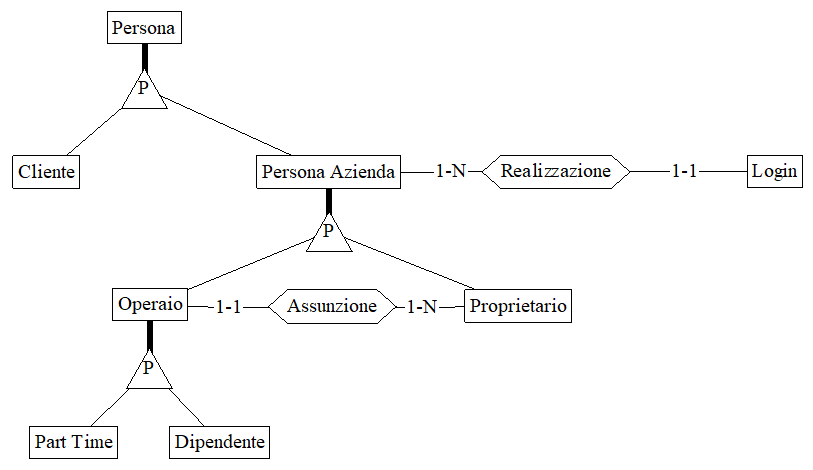
\includegraphics[width=0.8\textwidth]{img/Persone_Scheletro.png}
\end{figure}
\subsubsection{Schema Parziale}
Dopo l'inserimento degli attribuiti necessari per le varie entità, lo schema E/R parziale per  il proprietario e gli operai risulta essere il seguente:
\begin{figure}[htbp]
\centering
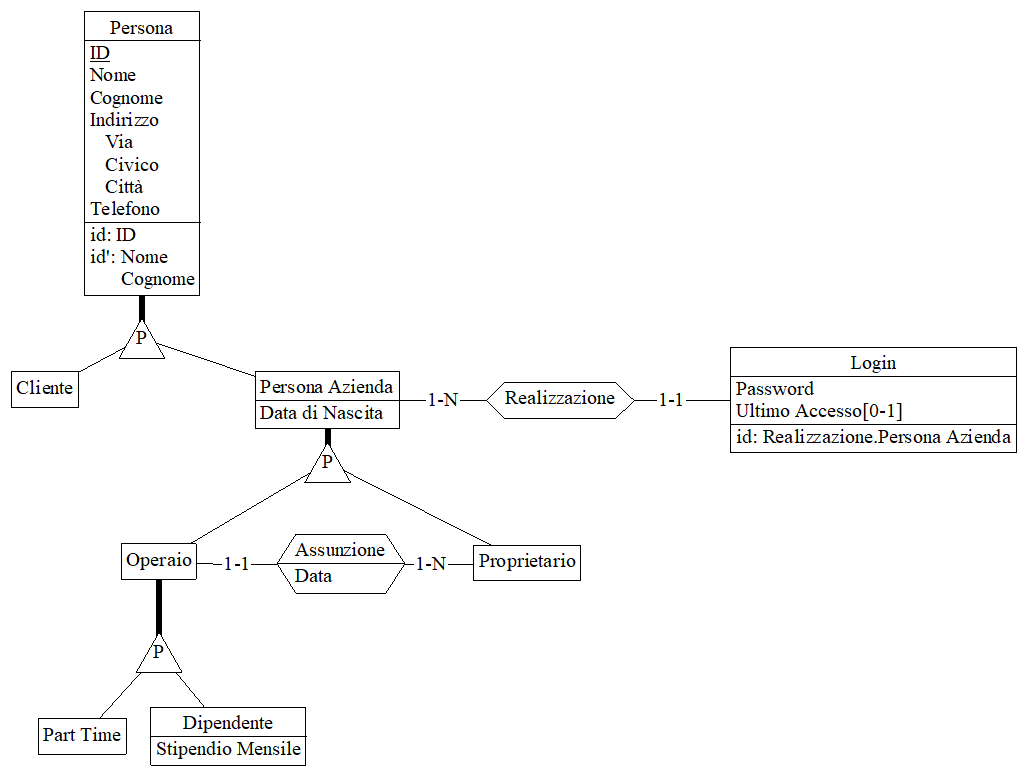
\includegraphics[width=0.8\textwidth]{img/Persone_Parziale.png}
\end{figure}
\newpage
\subsection{Fasi di Produzione}

\subsubsection{Schema scheletro}
Dopo aver esaminato i requisiti per le fasi della Produzione del Vino, si presenta il seguente schema scheletro:
\begin{figure}[htbp]
\centering
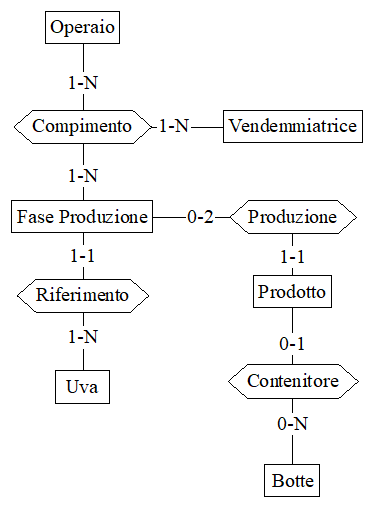
\includegraphics[width=0.7\textwidth]{img/Fasi_Scheletro}
\end{figure}
\subsubsection{Raffinamenti proposti}
La relazione \textit{Compimento} verrà convertita in entità e rinominata \textbf{Gruppo}, poiché come dai requisiti, è richiesto di memorizzare il gruppo degli operai per ogni fase di produzione.
L'entità Gruppo sarà identificata dal operaio e della fase di produzione.
\newline
\newline
L'entità \textbf{Fase Produzione} è una generalizzazione delle quattro fasi di produzione : \textbf{Raccolta, Pigiatura, Svinatura } e \textbf{Sfecciaura }, per cui tale entità verrà ridefinita in termini di queste sottoclassi.
\newline
\newline
L'entità \textbf{Prodotto} è una generalizzazione delle tipologie di prodotti : \textbf{Raspi, Mosto, Vinaccia, VNF, Feccia} e \textbf{Vino}, per cui tale entità verrà ridefinita in termini di queste sottoclassi.
\newpage 
\subsubsection{Schema Parziale}
Dopo l'applicazione dei raffinamenti proposti e l'inserimento degli attribuiti necessari per le varie entità, lo schema E/R parziale per le Fasi della Produzione del Vino risulta essere il seguente:
\begin{figure}[htbp]
\centering
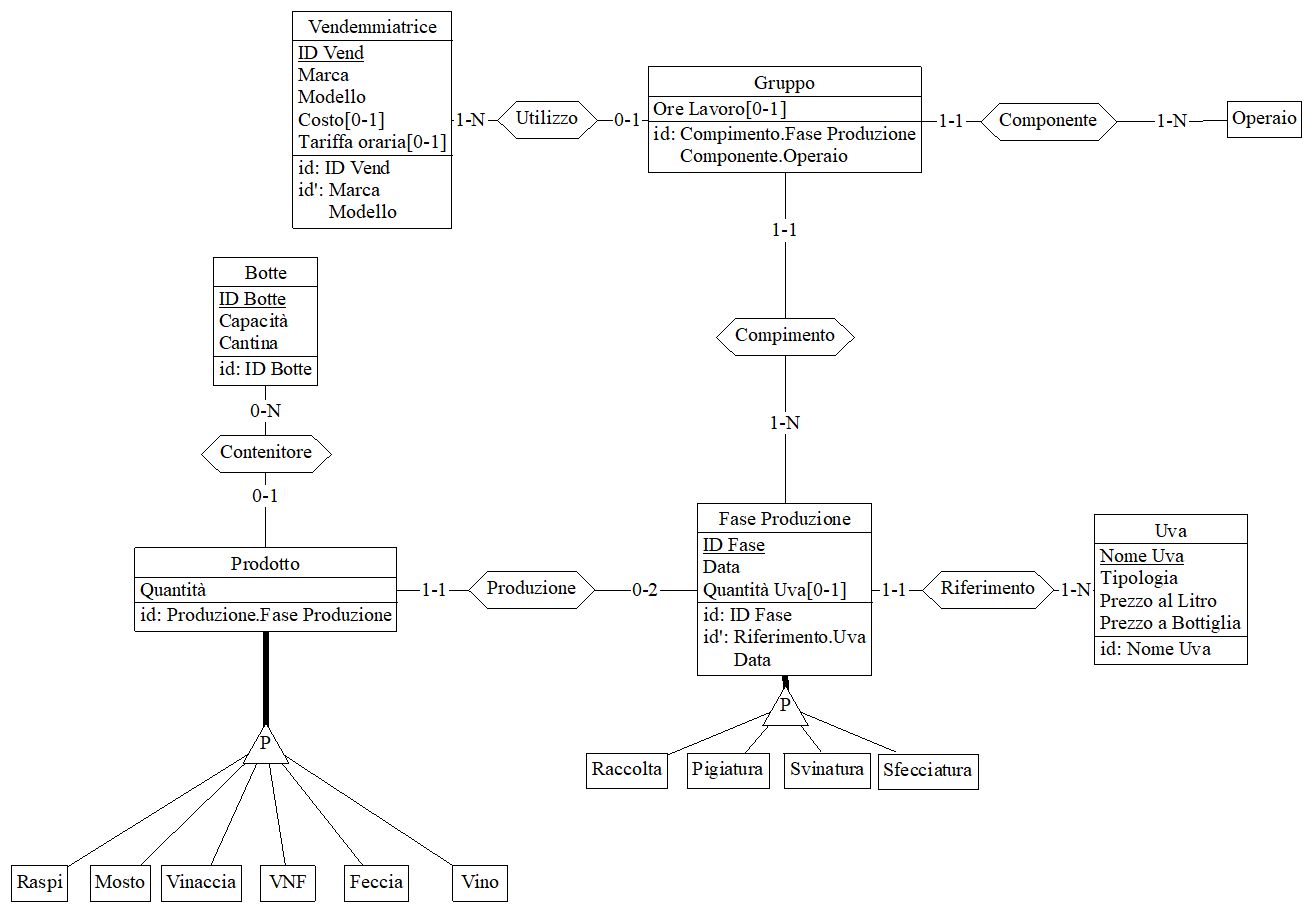
\includegraphics[width=1\textwidth]{img/Fasi_Parziale}
\end{figure}

\newpage
\subsection{Vendite}
\subsubsection{Schema scheletro}
Dopo aver esaminato i requisiti per lo storico della Vendite, si presenta il seguente schema scheletro:
\begin{figure}[htbp]
\centering
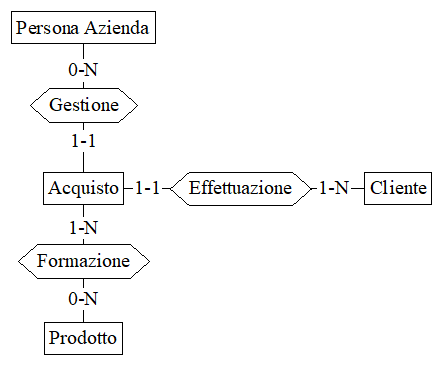
\includegraphics[width=0.7\textwidth]{img/Vendite_Scheletro}
\end{figure}
\subsubsection{Raffinamenti proposti}
L'entità \textbf{Prodotto} verrà sostituita con la sua sotto entità \textbf{Vino}, poiché come dai requisiti, è solo il Vino a essere venduto al cliente. Conseguentemente, la cardinalità minima della relazione \textit{Formazione} verrà cambiata da non obbligatoria a obbligatoria per ogni entità Vino.
\newline\newline
Dal momento che verrà fatto un acquisto da un specifico cliente, di tale acquisto si dovrà specificare la lista di vini acquistati, la modalità di acquisto, la relativa quantità e il relativo prezzo, quindi la relazione \textit{Formazione} viene rinominata in \textit{Dettaglio Acquisto}.
\subsubsection{Schema Parziale}
Dopo l'applicazione dei raffinamenti proposti e l'inserimento degli attribuiti necessari per le varie entità, lo schema E/R parziale per lo storico delle Vendite risulta essere il seguente:
\begin{figure}[htbp]
\centering
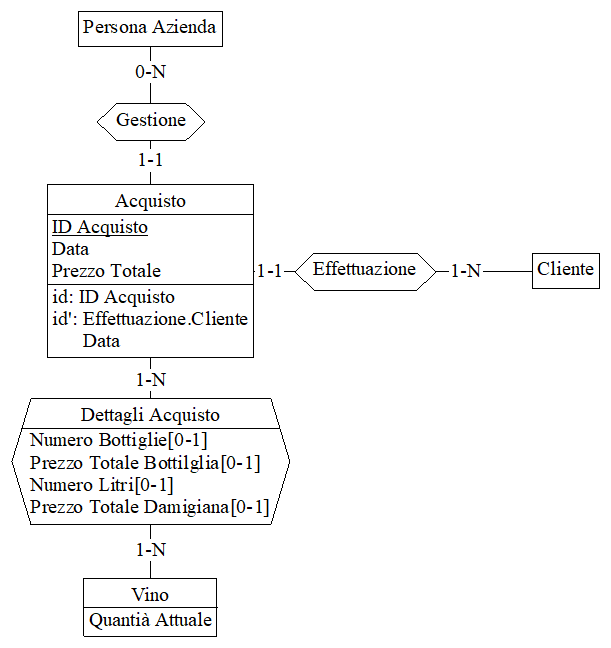
\includegraphics[width=0.7\textwidth]{img/Vendite_Parziale}
\end{figure}
\newpage
\subsection{Schema Finale}
Nella pagina successiva è presentato lo schema E/R finale.
\begin{figure}[htbp]
\centering
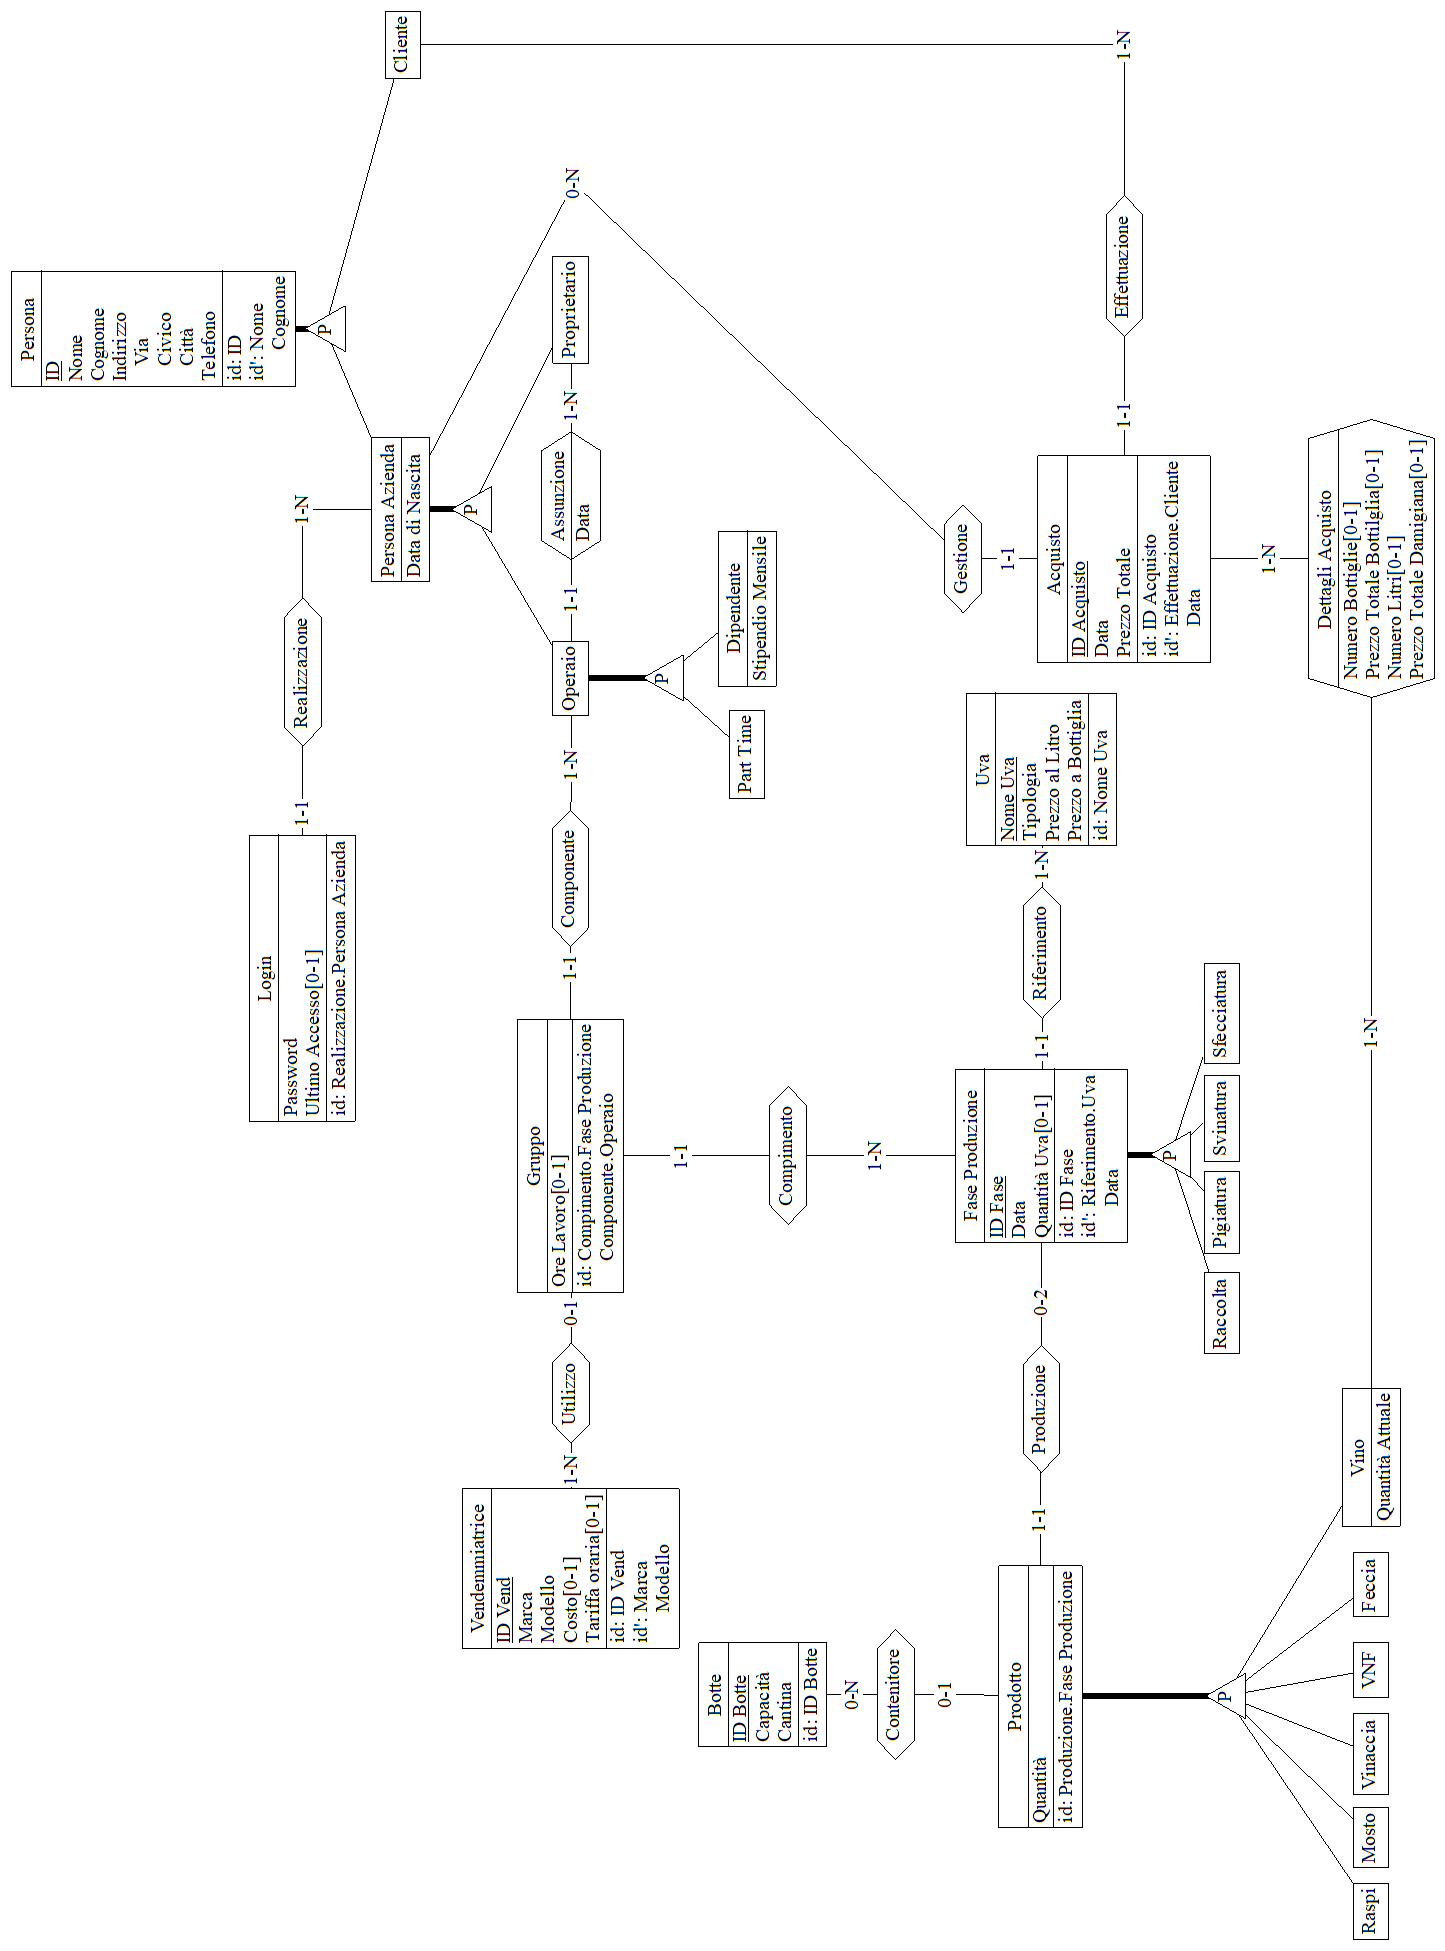
\includegraphics[height=25cm,width=1\textwidth]{img/Schema_Finale}
\end{figure}
\newpage
\section{Progettazione Logica}
\subsection{Stima del volume dei dati}
Si fornisce in questa fase una tabella che specifica il numero stimato di istanze per ogni entità e associazione dello schema concettuale finale.\
\newline
\newline
\begin{tabular}{p{0.35\textwidth} c c}\hline
    \textbf{Concetto} & \textbf{Costrutto}   & \textbf{Volume } \\\hline
    Login& E & 33\\\hline
    Persona &E& 133\\\hline
    Cliente & E & 100\\\hline
    Persona Azienda &E&33\\\hline
    Proprietario& E & 3\\\hline
    Operaio& E & 30\\\hline
    Dipendente& E & 10  \\\hline
    Part-Time& E & 20 \\\hline
    Gruppo& E & 100\\\hline
    Vendemmiatrice& E & 10\\\hline
    Fase Produzione & E & 400\\\hline
    Raccolta & E & 100\\\hline
    Pigiatura & E & 100\\\hline
    Svinatura & E &  100\\\hline
    Sfecciatura & E & 100 \\\hline
    Uva & E & 10\\\hline
    Prodotto & E & 600\\\hline
    Raspi & E & 100\\\hline
    Mosto& E & 100\\\hline
     Vinaccia& E &100 \\\hline
    VNF& E & 100\\\hline
    Feccia& E & 100\\\hline
    Vino & E & 100\\\hline
    Botte & E & 50\\\hline
    Acquisto & E & 300\\\hline
    Assunzione & R & 30\\\hline
    Gestione & R & 300\\\hline
    Componente & R & 100\\\hline
    Utilizzo & R & 100\\\hline
    Compimento & R &  100\\\hline
    Riferimento & R & 400\\\hline
    Produzione & R & 600\\\hline
    Contenitore & R & 500\\\hline
    Dettagli Acquisto & R & 3000\\\hline
    Effettuazione & R & 300\\\hline
    Realizzazione & R & 33\\\hline
\end{tabular}
\newline
\textit{\textbf{Tabella 3.1.1}  - Tabella dei Volumi.}
\newpage
\subsection{Descrizione delle operazioni principali e stima della loro frequenza} 
In questa fase si propone una tabella delle operazioni utilizzata per costituire una stima delle principali operazioni.\\
\newline
\newline
\begin{tabular}{p{0.05\textwidth} |p{0.5\textwidth}| p{0.2\textwidth}| c}\hline
    \textbf{N.} & \textbf{Operazione eseguite da una persona} & \textbf{Frequenza}  & \textbf{Tipo} \\\hline
    1&Inserimento Operaio & 10 all'anno & I \\\hline
    2&Inserimento Uva & 1 all'anno & I\\\hline
    3&Inserimento Vendemmiatrice & 1 all'anno & I\\\hline
    4&Inserimento Botte & 3 all'anno & I\\\hline
    5&Inserimento Cliente & 1 al giorno& I\\\hline
    6&Inserimento Fasi Produzione & 10 all'anno & I\\\hline
    7&Inserimento Prodotto & 10 all'anno &I \\\hline
    8&Inserimento Gruppo & 10 all'anno  &I \\\hline
    9&Registrazione Acquisto & 5 al giorno & I \\\hline
    10&Visualizzazione delle informazioni basilari di un vino (data, quantità e botte) di un data uva &5 al giorno & B\\\hline
    11&Visualizzazione delle informazioni basilari (uva, quantita, botte) dei prodotti di una data fase di un dato anno& 2 volte all'anno & B\\\hline
    12&Visualizzazione dei gruppi di ogni fase con componente uno specifico operaio Part-time e il relativo calcolo delle ore complessive di lavoro& 1 volta all'anno&B\\\hline
    13&Visualizzazione di tutti gli acquisti di un dato cliente e calcolo della spesa complessiva & 1 volta a settimana&B\\\hline
\end{tabular}
\newline
\textit{\textbf{Tabella 3.2.1}  - Tabella delle Operazioni delle Persone.}
\newline
\newline
\newline
\begin{tabular}{p{0.05\textwidth} |p{0.5\textwidth}| p{0.2\textwidth}| c}\hline
    \textbf{N.} & \textbf{Operazione eseguite dal sistema software} & \textbf{Frequenza}  & \textbf{Tipo} \\\hline
    1&Inserimento Login & 10 all'anno & I \\\hline
    2&Modifica della data di ultimo Login& 5 al giorno & I\\\hline
    3&Visualiazzazione dei dati di accesso per una data persona che lavora nell'azienda (Proprietario e Operai) per verificarne la correttezza & 5 al giorno &B \\\hline
\end{tabular}
\newline
\textit{\textbf{Tabella 3.2.1}  - Tabella delle Operazioni del Sistema Software.}

\newpage
\subsection{Schemi di navigazione e tabelle degli accessi}
Dopo aver determinato il volume dei dati ed aver associato a ciascuna operazione principale richiesta la propria frequenza di esecuzione, si procede determinando lo schema di navigazione di riferimento per le principali operazioni richieste e si associa ad ognuna di essa anche la relativa tavola degli accessi. Le operazioni per cui questo passaggio risulta essere banale non verranno considerate. Nel calcolo degli accessi si stima come doppio il peso degli accessi in scrittura, rispetto a quelli in lettura.

\begin{itemize}
\item Registrazione Acquisto\\
\newline
Inserimento di un acquisto effettuato da un dato cliente. Per ogni acquisto la quantità di vino diminuisce.\\
\newline
\begin{figure}[htbp]
\centering
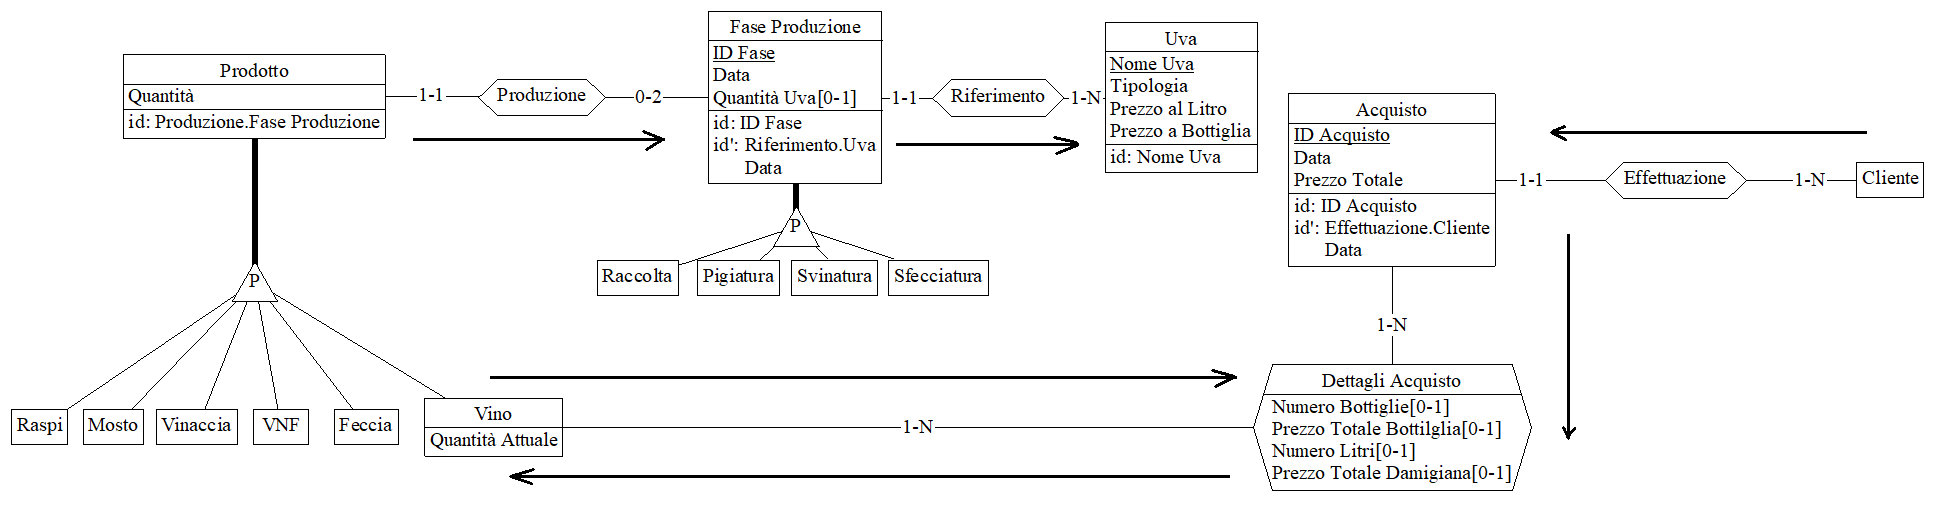
\includegraphics[width=1\textwidth]{img/vendite_accessi.png}
\end{figure}
\newline
\newline
\begin{tabular}{c|c|c|c}\hline
    \textbf{Concetto} & \textbf{Costrutto} &  \textbf{Accesso} & \textbf{Tipo} \\\hline
    Cliente & E & 1 & L\\\hline
    Effettuare & R& 1 & S \\\hline
    Acquisto & E & 1 & S\\\hline
    Dettagli Acquisto &R & 3000/300 = 10 & S\\\hline
    Vino & E & 3000/300 = 10 & L\\\hline
    Vino & E & 3000/300 = 10 & S\\\hline
    Produzione & R& 3000/300 = 10 & L\\\hline
    Fase Produzione & E & 3000/300 = 10& L\\\hline
    Riferimento & R&3000/300 = 10 & L\\\hline
    Uva& E & 3000/300 = 10& L\\\hline
\end{tabular}
\newline
Totale: 6L + 4S \qquad \qquad Frequenza operazione: 5 al giorno
\newline
\newline
\textbf{Totale costo}: 5 * (6 + 4*2) = 70 al giorno \\
\newpage
\item Visualizzazione delle informazioni basilari (uva, quantita, botte) dei prodotti di una data fase di un dato anno \\
\newline
\begin{figure}[htbp]
\centering
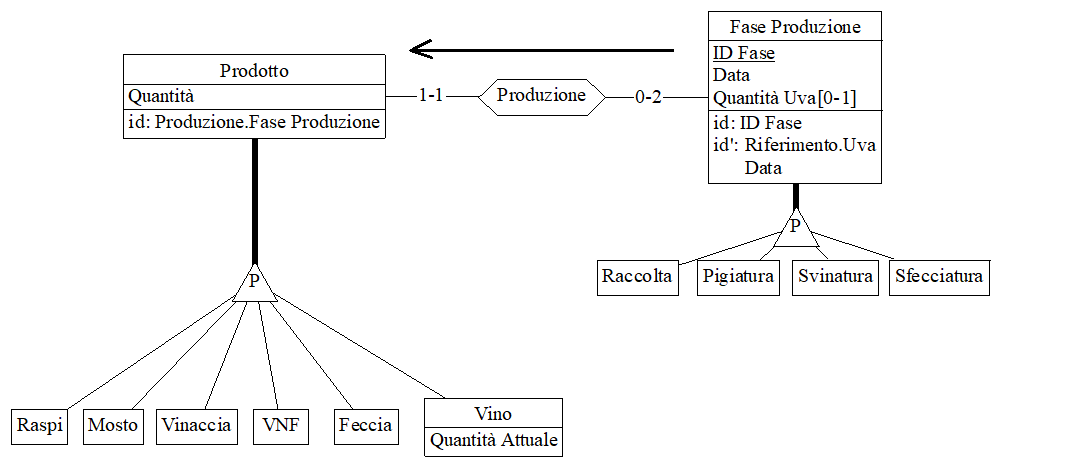
\includegraphics[width=1\textwidth]{img/prodotti_accessi.png}
\end{figure}
\newline
\newline
\begin{tabular}{c|c|c|c}\hline
    \textbf{Concetto} & \textbf{Costrutto} &  \textbf{Accesso} & \textbf{Tipo} \\\hline
    Fase Produzione & E & 1 & L\\\hline
    Produzione & R& 600/400 = 2 & L \\\hline
    Prodotti & E & 600/400 = 2 & L\\\hline
\end{tabular}
\newline
Totale: 5L \qquad \qquad Frequenza operazione: 2 all'anno
\newline
\newline
\textbf{Totale costo}: 2 * 5 = 10 all'anno\\
\newpage
\item Visualizzazione dei gruppi di ogni fase con componente uno specifico operaio Part-time e il relativo calcolo delle ore complessive di lavoro
\newline
\begin{figure}[htbp]
\centering
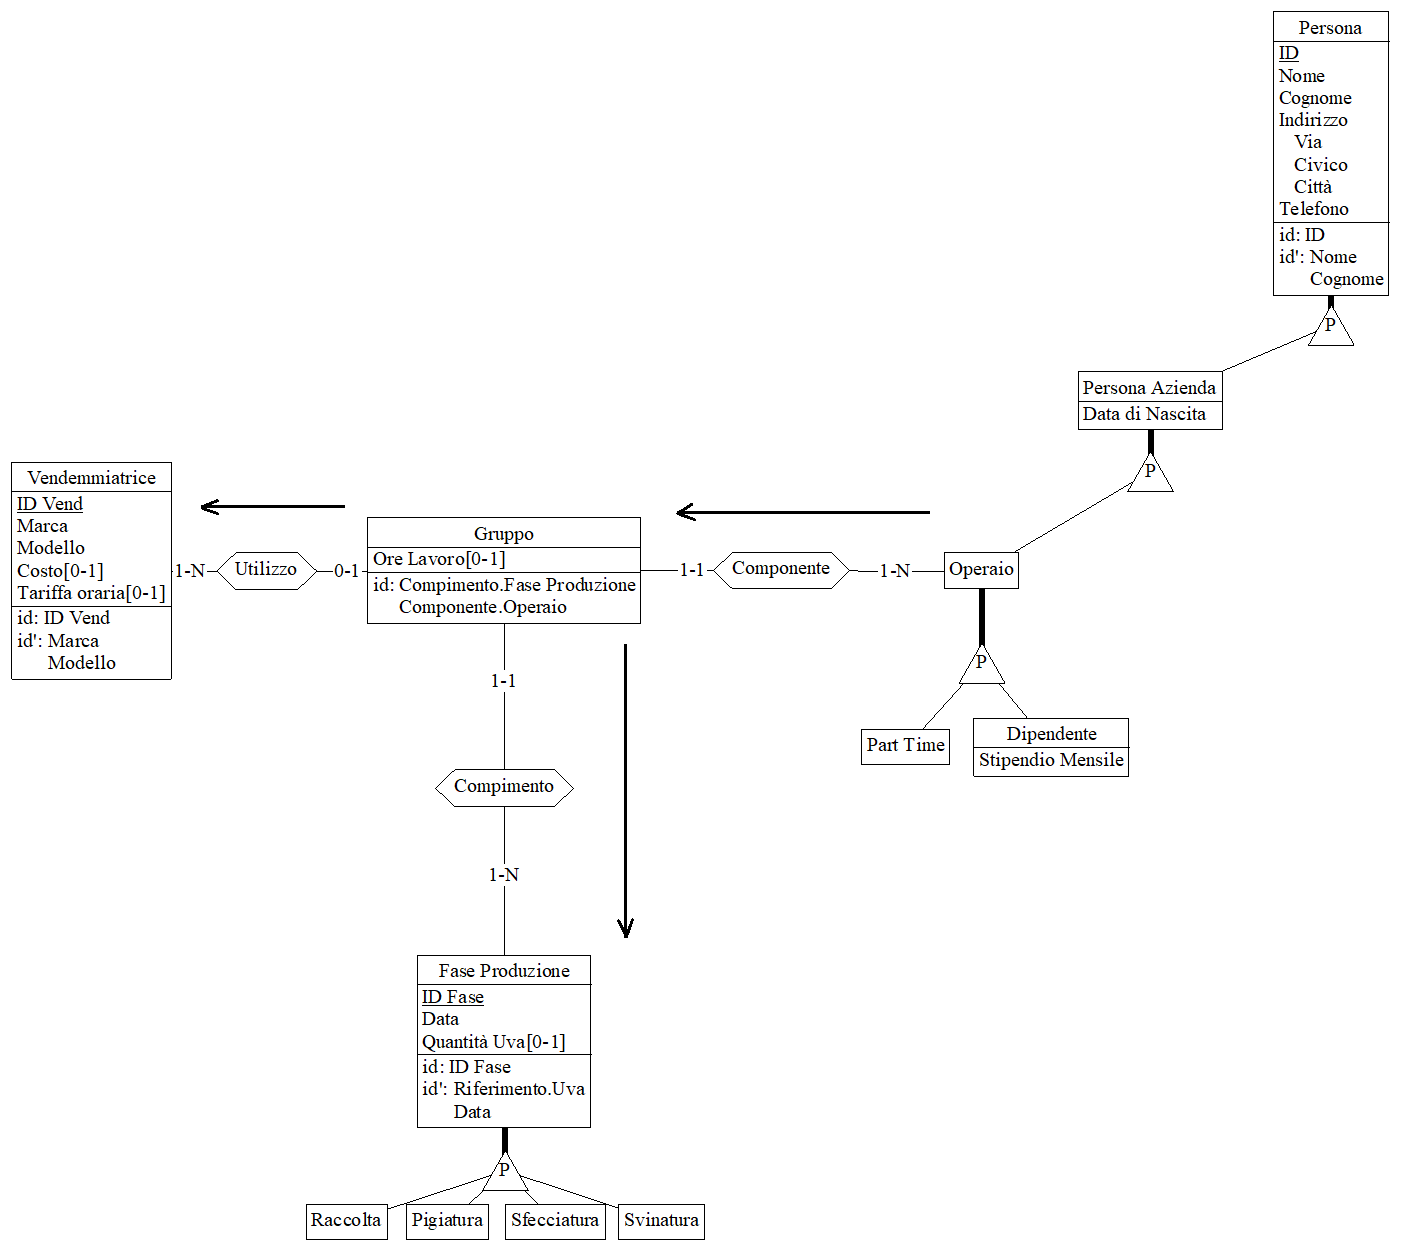
\includegraphics[width=1\textwidth]{img/parttime_accessi.png}
\end{figure}
\newline
\newline
\begin{tabular}{c|c|c|c}\hline
    \textbf{Concetto} & \textbf{Costrutto} &  \textbf{Accesso} & \textbf{Tipo} \\\hline
    Operaio & E & 1 & L\\\hline
    Componente & R&  100/30 = 3 & L \\\hline
    Gruppo & E &  100/30 = 3 & L\\\hline
    Compimento & R& 100/30 = 3 & L \\\hline
    Fase Produzione& E & 100/30 = 3 & L\\\hline
    Utilizzo & R& 100/30 = 3 & L \\\hline
    Vendemmiatrice& E &  100/30 = 3 & L\\\hline
\end{tabular}
\newline
Totale: 19L \qquad \qquad Frequenza operazione: 1 all'anno
\newline
\newline
\textbf{Totale costo}: 1 * 19 = 19 all'anno\\
\end{itemize}
\newpage
\subsection{Analisi delle ridondanze}
Nello schema E/R riferito alle vendite sono presenti delle ridondanze. 
Infatti l'attributo Prezzo dell'entità Acquisto è un attributo derivabile, dai due attributi ( Prezzo Totale Damigiana e Prezzo Totale Bottiglia ) della relazione Dettaglio Acquisto.
Anch'essi sono derivabili da attributi che sono presenti nell'entità Uva ( Prezzo al Litro e Prezzo a Bottiglia )e nella stessa relazione (Numero Litri e Numero Bottiglie).
Considerando le operazioni eseguibili, mantenere gli attributi o toglierli comporta solamente uno spreco del tutto trascurabile di memoria, si decide quindi di mantenerli per semplicità. 
\newpage
\subsection{Raffinamento dello schema}
\begin{itemize}
\item \textbf{Eliminazione delle gerarchie} \\
Nello schema E/R compaiono in tutto cinque gerarchie da eliminare.\\
\newline
Per la gerarchia OPERAIO, si decide di adottare come soluzione il collasso verso l'alto. La scelta è motivata dal fatto che nonostante debba essere aggiunto un singolo attributo “Tipologia” alla tabella OPERAIO e quindi uno spreco di memoria per la presenza di valori nulli, la scelta assicura un numero minore di accessi rispetto alle altre nelle quali le occorrenze e gli attributi sono distinti tra le varie entità.\\
\begin{figure}[htbp]
\centering
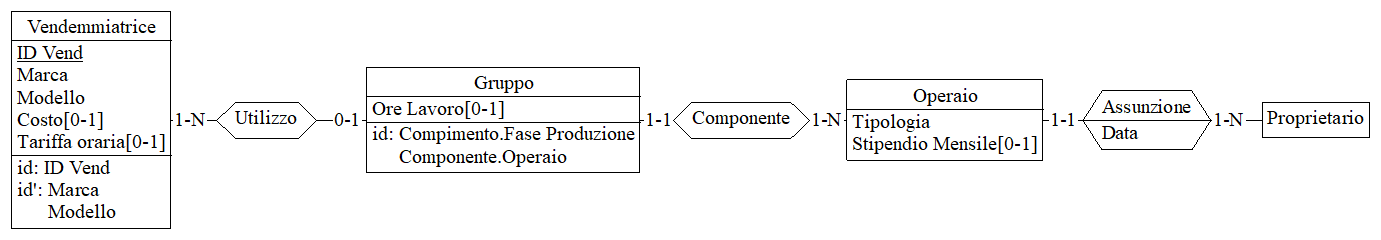
\includegraphics[width=1\textwidth]{img/eliminazione_ger_Operaio.png}
\end{figure}\\\newline\newline

Per gli stessi motivi si utilizza il collasso verso l’alto anche per eliminare la gerarchia PERSONA AZIENDA.
\begin{figure}[htbp]
\centering
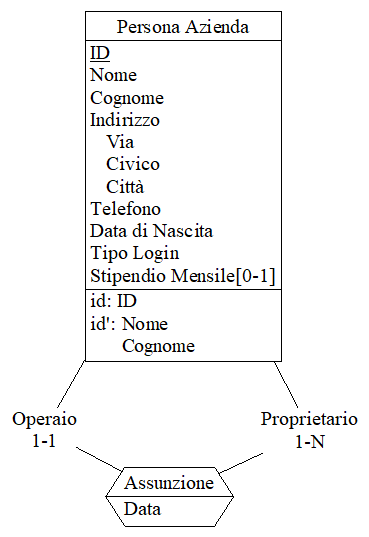
\includegraphics[width=0.5\textwidth]{img/eliminazione_ger_PersonaAzienda.png}
\end{figure}\\\newline\newline

Per la gerarchia PERSONA, si decide di adottare come soluzione il collasso verso il basso. La scelta è motivata dal fatto che le entità PERSONA AZIENDA e CLIENTE si riferiscono solo a occorrenze di entità differenti.In tal caso c'è risparmio di memoria rispetto al collasso verso l'alto, perché, in linea di principio, gli attributi non assumono mai valori nulli.\\
\begin{figure}[htbp]
\centering
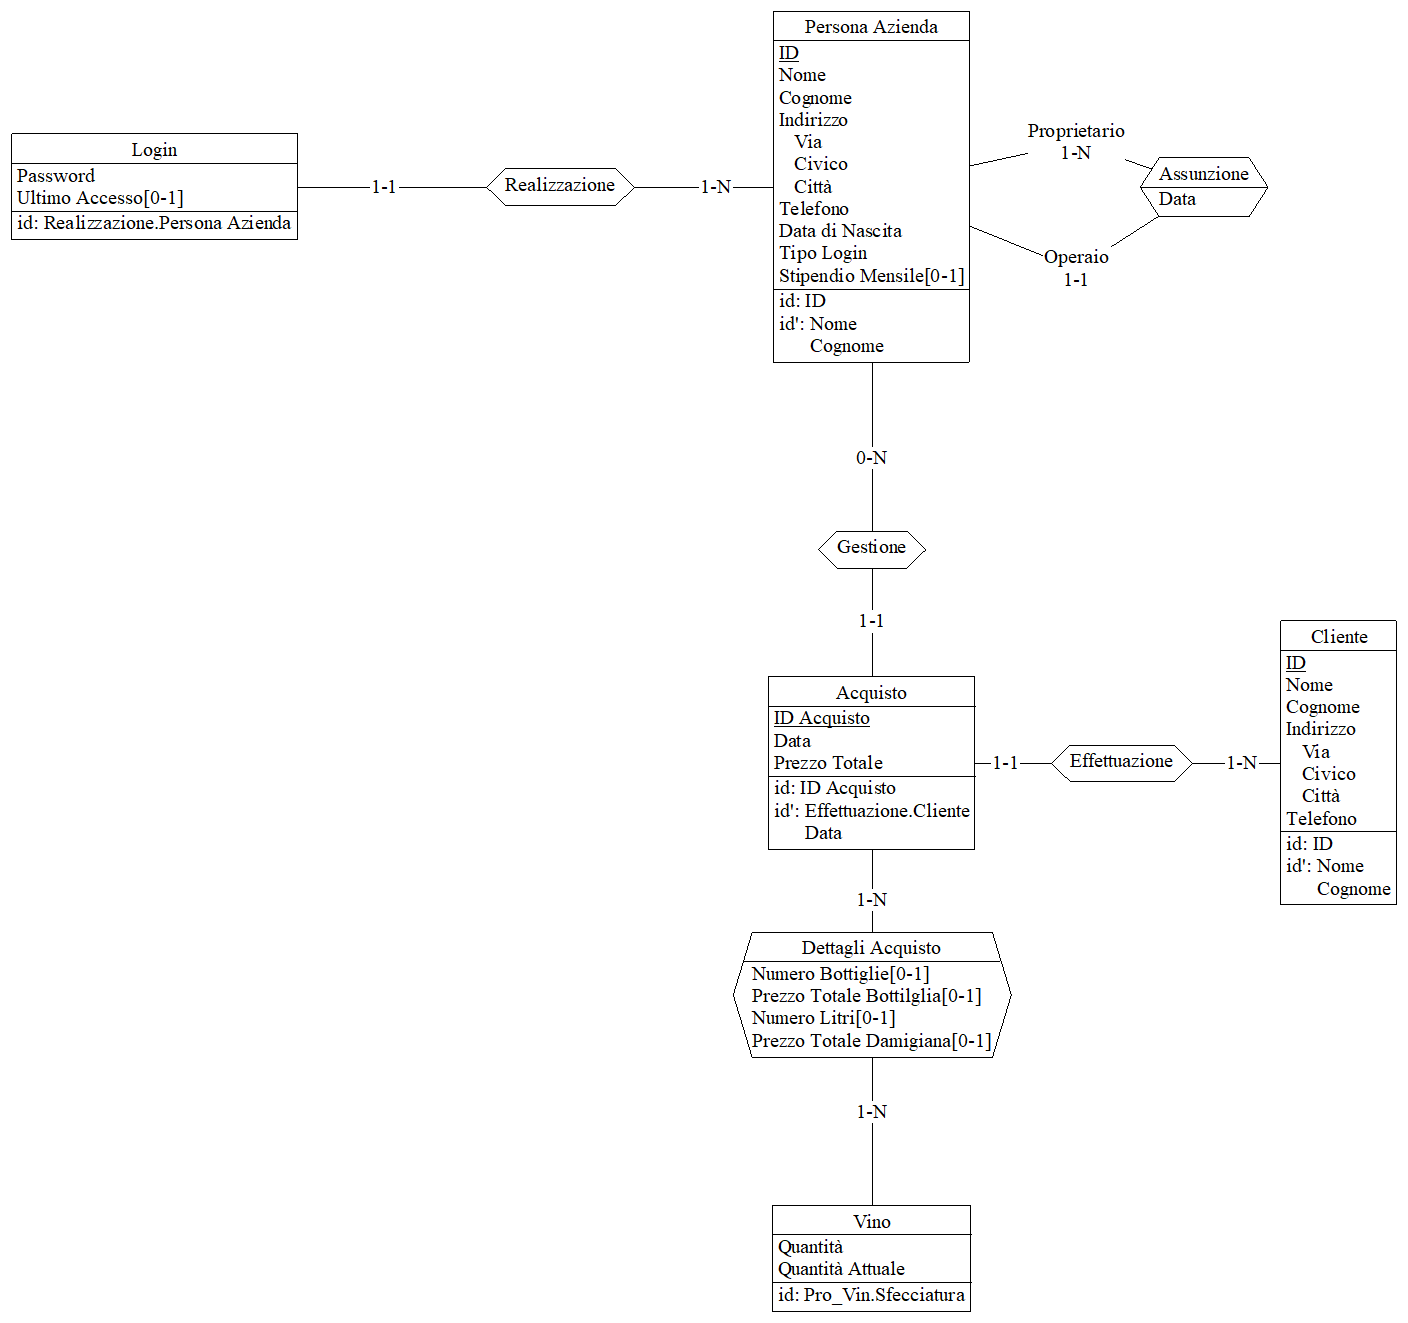
\includegraphics[width=0.95\textwidth]{img/eliminazione_ger_Persona.png}
\end{figure}\\\newline\newline
\newpage
Per la gerarchia PRODOTTO e FASE PRODUZIONE, si decide di adottare come soluzione il collasso verso il basso. La scelta è motivata dal fatto che la frequenza delle operazioni eseguite su queste due entità sono relativamente basse e quindi si vuole privilegiare la  eliminazione di eventuali valori nulli e quindi la riduzione di memoria utilizzata, piuttosto che le prestazioni.\\
Cosi facendo però l'entità GRUPPO si divide per ogni fase, ma è un bene poiché l'entità VENDEMMIATRICE è riferita solo al GRUPPO che effettua la fase RACCOLTA.\newline
\newline
\begin{figure}[htbp]
\centering
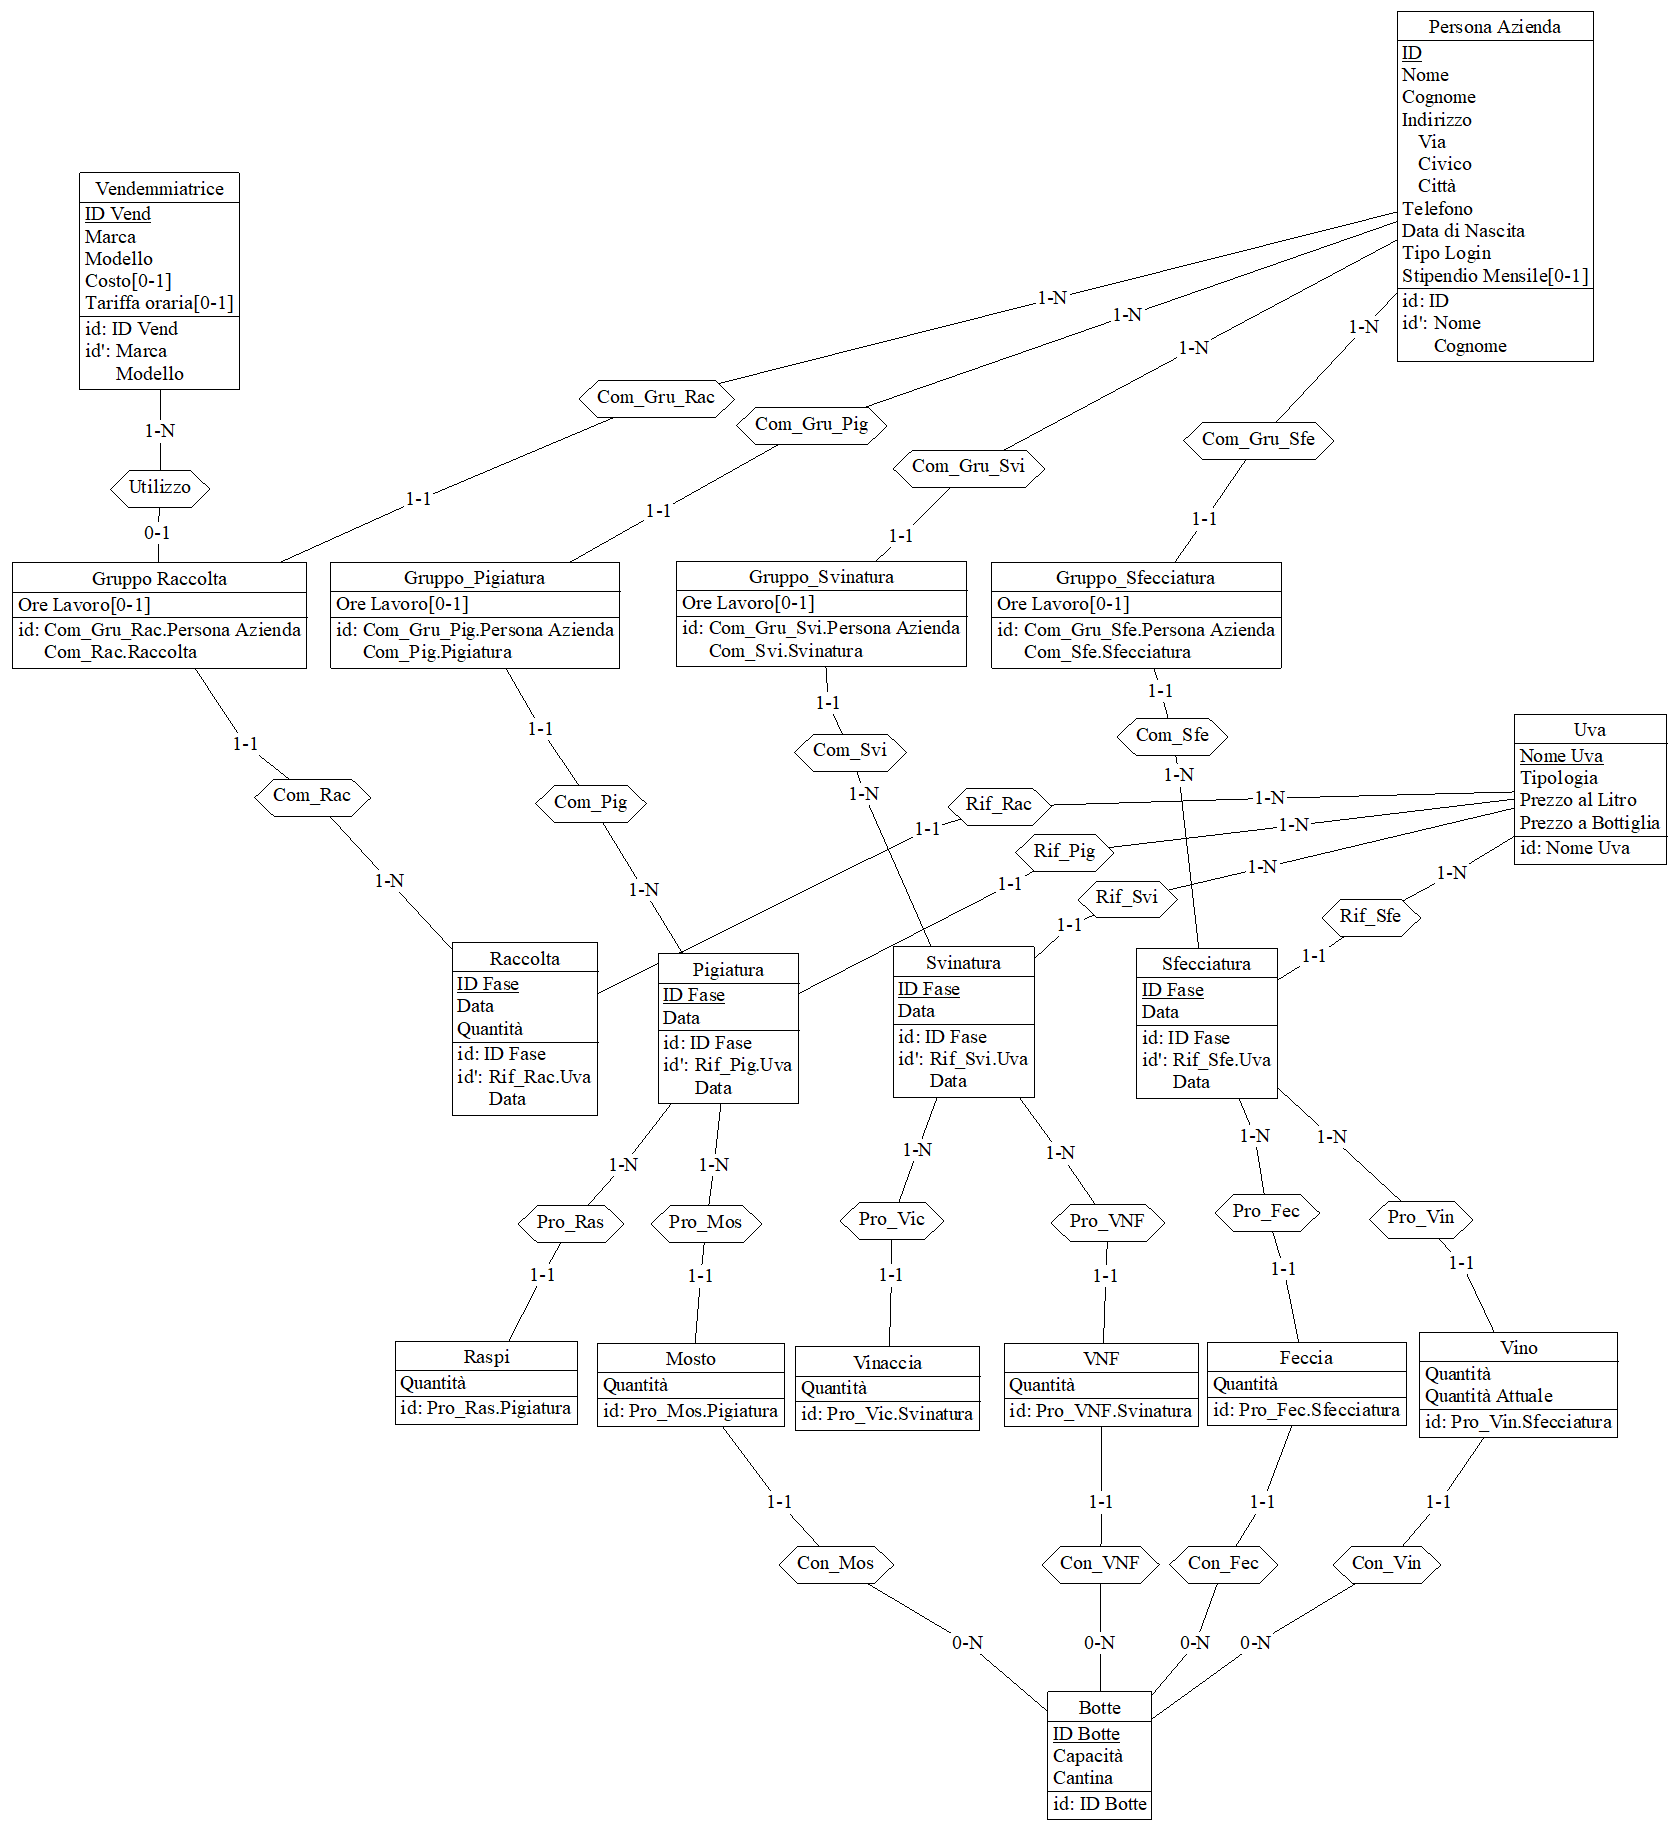
\includegraphics[width=1\textwidth]{img/eliminazione_ger_prodotto_fase.png}
\end{figure}\\
\item \textbf{Eliminazione degli  attributi composti}\\
\'E possibile individuare nello schema E/R che l’attributo “Indirizzo” delle entità PERSONA è un attributo composto dai sotto-attributi: “Via”, ”Civico”, ”Città”. Esso viene quindi scomposto nelle sue tre sotto-parti per entrambe le entità in questione.\\
\item \textbf{Scelta delle chiavi primarie}\\
Nello schema E/R proposto sono già evidenziate tutte le chiave primarie.\\
Per l'entità \textit{Persona} e  \textit{Botte} è richiesto dalle specificahe un numero identificativo.\\
L'entità seguenti 
\begin{itemize}
\item  \textit{Vendemmiatrice}
\item  \textit{Fase Produzione} 
\item  \textit{Cliente}
\item  \textit{Acquisto}
\end{itemize} 
verrebbero identificate tramite una composizione di attributi. Poiché risulta scomodo utilizzare una chiave primaria composta, soprattutto quando deve essere usata come chiave esterna, si opta per una chiave primaria più semplice, composta dal solo attributo numerico.\\
L' entità \textit{Uva} è identificata con il Nome della stessa, poichè non ci saranno mai due uve con lo stesso nome.\\
L' entità \textit{Login} è identificata dalla chiave dell'entità  \textit{Persona} .\\
L' entità \textit{Prodotto}  è identificata dalla chiave dell'entità  \textit{Fase Produzione}.\\
L' entità \textit{Gruppo} è identificata dalle chiave dell'entità \textit{Operaio} e della entità \textit{Fase Produzione} .\\
\end{itemize}
\subsection{Traduzione di entità e associazioni in relazioni}
\textbf{PERSONA\_AZIENDA}(\underline{ID},Nome, Cognome, Ind\_Via, Ind\_Civico, Ind\_Citta, Telefono, Data\_di\_Nascita, Tipo\_Login, Stipendio\_Mensile*)\\
AK: Nome, Cognome\\\newline
\textbf{ASSUNZIONE}(\underline{ID\_Operaio}, ID\_Proprietario, Data)\\
FK: ID\_Operaio REFERENCES \textbf{PERSONA\_AZIENDA}\\
FK: ID\_Proprietario REFERENCES \textbf{PERSONA\_AZIENDA}\\\newline
\textbf{LOGIN }(\underline{ID\_Aziendale},Password,Ultimo Accesso*)\\
FK: IDAziendale REFERENCES \textbf{PERSONA\_AZIENDA}\\\newline
\textbf{UVA}(\underline{Nome\_Uva}, Tipologia, Prezzo\_al\_Litro, Prezzo\_a\_Bottiglia)\\\newline
\textbf{VENDEMMIATRICE}(\underline{ID\_Vend}, Marca, Modello, Costo*,Tariffa\_oraria*)\\
AK: Marca, Modello\\\newline
\textbf{BOTTE}(\underline{ID\_Botte}, Capacita, Cantina)\\\newline
\textbf{RACCOLTA }(\underline{ID\_Fase}, Data, Uva, Quantita)\\
FK: Uva REFERENCES \textbf{UVA}\\
AK: Uva, Data \\\newline
\textbf{PIGIATURA }(\underline{ID\_Fase}, Data, Uva)\\
FK: Uva REFERENCES \textbf{UVA}\\
AK: Uva, Data \\\newline
\textbf{SVINATURA }(\underline{ID\_Fase}, Data, Uva)\\
FK: Uva REFERENCES \textbf{UVA}\\
AK: Uva, Data \\\newline
\textbf{SFECCIATURA }(\underline{ID\_Fase}, Data, Uva)\\
FK: Uva REFERENCES \textbf{UVA}\\
AK: Uva, Data \\\newline
\textbf{RASPI }(\underline{ID\_Pigiatura}, Quantita )\\
FK: ID\_Pigiatura REFERENCES \textbf{PIGIATURA}\\\newline
\textbf{MOSTO}(\underline{ID\_Pigiatura},  Quantita, Botte)\\
FK: ID\_Pigiatura REFERENCES \textbf{PIGIATURA}\\
FK: Botte REFERENCES \textbf{BOTTE}\\\newline
\textbf{VINACCIA}(\underline{ID\_Svinatura},  Quantita)\\
FK: ID\_Svinatura REFERENCES \textbf{SVINATURA}\\\newline
\textbf{VNF}(\underline{ID\_Svinatura},  Quantita, Botte)\\
FK: ID\_Svinatura REFERENCES \textbf{SVINATURA}\\
FK: Botte REFERENCES \textbf{BOTTE}\\\newline
\textbf{FECCIA}(\underline{ID\_Sfecciatura},  Quantita, Botte)\\
FK: ID\_Sfecciatura REFERENCES \textbf{SFECCIATURA}\\
FK: Botte REFERENCES \textbf{BOTTE}\\\newline
\textbf{VINO}(\underline{ID\_Sfecciatura},  Quantita, Quantita\_Attuale,Botte)\\
FK: ID\_Sfecciatura REFERENCES \textbf{SFECCIATURA}\\
FK: Botte REFERENCES \textbf{BOTTE}\\\newline
\textbf{GRUPPO\_RACCOLTA}(\underline{ID\_Raccolta}, \underline{ID\_Operaio}, Ore\_Lavoro *, ID\_Vendemmiatrice*)\\
FK: ID\_Raccolta REFERENCES \textbf{RACCOLTA}\\
FK: ID\_Operaio REFERENCES \textbf{PERSONA\_AZIENDA}\\
FK: ID\_Vendemmiatrice REFERENCES \textbf{VENDEMMIATRICE}\\\newline
\textbf{GRUPPO\_PIGIATURA}(\underline{ID\_Pigiatura}, \underline{ID\_Operaio}, Ore\_Lavoro *)\\
FK: ID\_Pigiatura REFERENCES \textbf{PIGIATURA}\\
FK: ID\_Operaio REFERENCES \textbf{PERSONA\_AZIENDA}\\\newline
\textbf{GRUPPO\_SVINATURA}(\underline{ID\_Svinatura}, \underline{ID\_Operaio}, Ore\_Lavoro *)\\
FK: ID\_Svinatura REFERENCES \textbf{SVINATURA}\\
FK: ID\_Operaio REFERENCES \textbf{PERSONA\_AZIENDA}\\\newline
\textbf{GRUPPO\_SFECCIATURA}(\underline{ID\_Sfecciatura}, \underline{ID\_Operaio}, Ore\_Lavoro *)\\
FK: ID\_Sfecciatura REFERENCES \textbf{SFECCIATURA}\\
FK: ID\_Operaio REFERENCES \textbf{PERSONA\_AZIENDA}\\\newline
\textbf{CLIENTE}(\underline{ID\_Cliente},Nome, Cognome, Ind\_Via, Ind\_Civico, Ind\_Citta, Telefono)\\
AK: Nome, Cognome\\\newline
\textbf{ACQUISTO}(\underline{ID\_Acquisto}, Data, ID\_Cliente, ID\_Aziendale, Prezzo\_Totale)\\
FK: ID\_Cliente REFERENCES \textbf{CLIENTE}\\
FK: ID\_Aziendale REFERENCES \textbf{PERSONA\_AZIENDA}\\
AK: ID\_Cliente, Data\\\newline
\textbf{DETTAGLI\_ACQUISTO}(\underline{ID\_Acquisto}, \underline{ID\_Vino}, Numero\_Bottiglie*, Prezzo\_Totale\_Bottiglie*, Numero\_Litri *,  Prezzo\_Totale\_Damigiana*)\\
FK: ID\_Acquisto REFERENCES \textbf{ACQUISTO}\\
FK: ID\_Vino REFERENCES \textbf{VINO}
\subsection{Schema relazionale finale}
\begin{figure}[htbp]
\centering
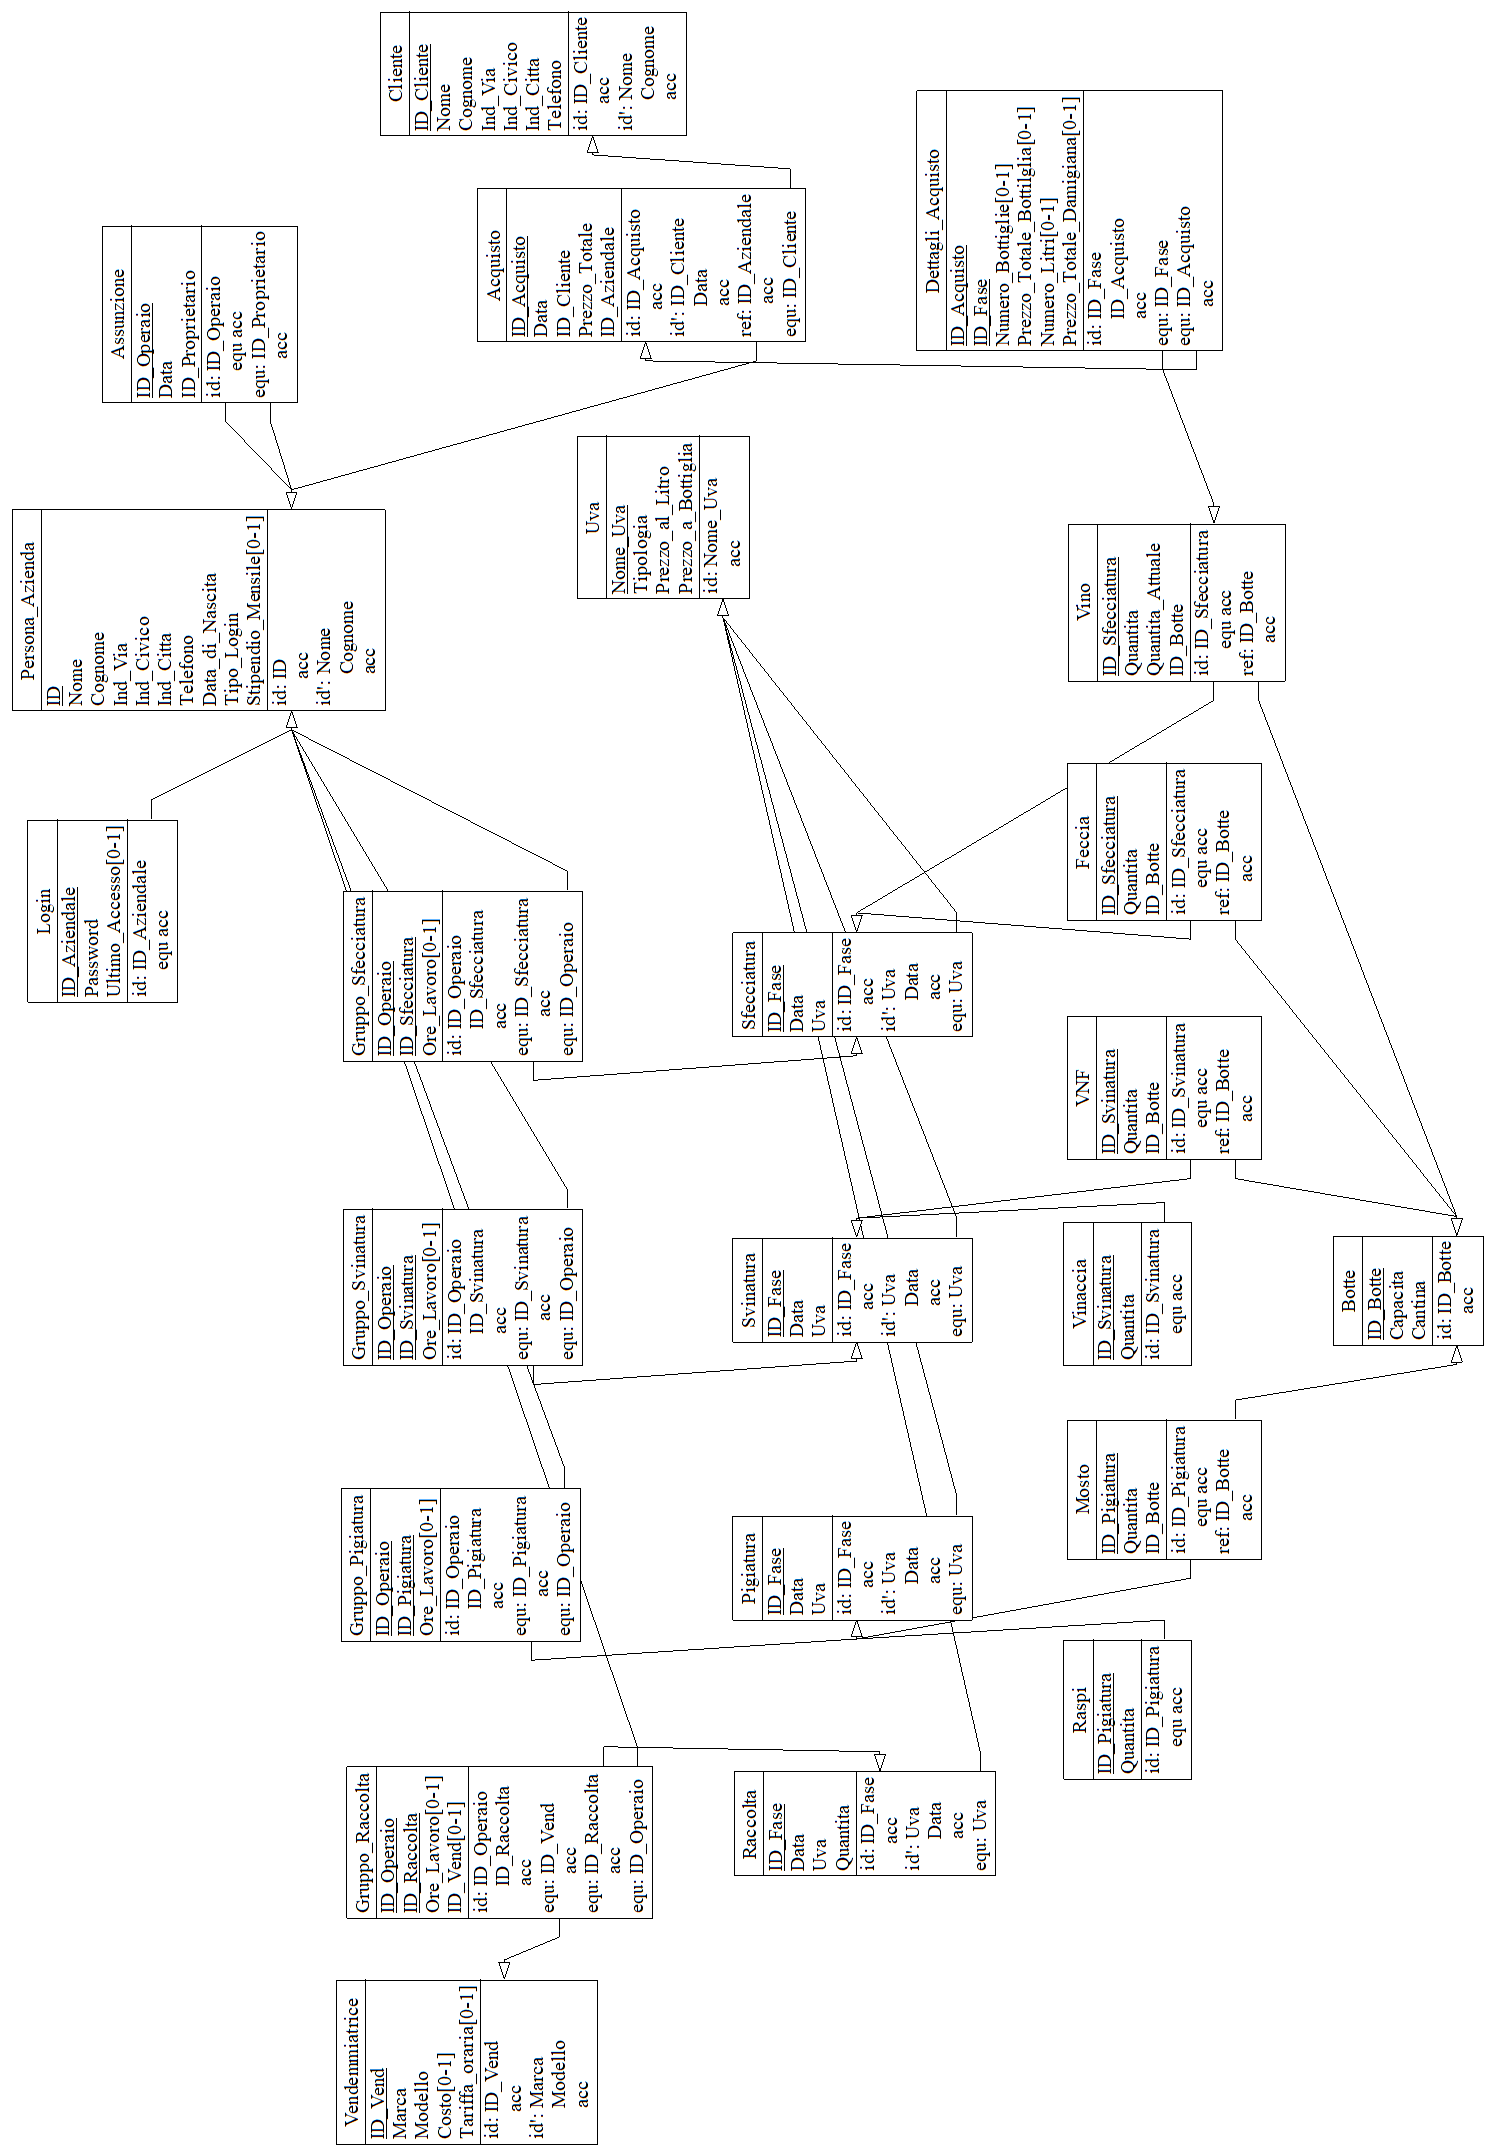
\includegraphics[height=25cm,width=1\textwidth]{img/Schema_Finale_Logica}
\end{figure}
\newpage
\subsection{Traduzione delle operazioni in query SQL}
\begin{itemize}
\item \textbf{Inserimento Operaio}\\\newline
INSERT INTO Persona\_Azienda(Nome, Cognome, Ind\_Via, Ind\_Civico, Ind\_Citta, Telefono, Data\_di\_Nascita, Tipo\_Login, Stipendio\_Mensile)  VALUES (?, ?, ?, ?, ?, ?, ?, ?, ?, ?)\\\newline
SELECT ID FROM PERSONA\_AZIENDA WHERE Nome = ? AND Cognome = ?\\\newline
INSERT INTO Assunzione(ID\_Operaio, Data, ID\_Proprietario)  VALUES (?, ?, ?)\\\newline
\item \textbf{Inserimento Uva}\\\newline
INSERT INTO Uva(Nome\_Uva, Tipologia, Prezzo\_al\_Litro, Prezzo\_a\_Damigiana) VALUES (?, ?, ?, ?)\\\newline
\item \textbf{Inserimento Vendemmiatrice}\\\newline
Se è stata acquistata:  \\
INSERT INTO Vendemmiatrice(ID\_Vend, Marca, Modello, Costo ) VALUES (?, ?, ?, ?)\\\newline
Se è stata presa in prestito:\\
INSERT INTO Vendemmiatrice(ID\_Vend, Marca, Modello, Tariffa\_oraria ) VALUES (?, ?, ?, ?)\\\newline
\item \textbf{Inserimento Botte}\\\newline
INSERT INTO Botte(ID\_Botte, Capacita, Cantina) VALUES (?, ?, ?)\\\newline
\item \textbf{Inserimento Cliente}\\\newline
INSERT INTO Cliente(Nome, Cognome, Ind\_Via, Ind\_Civico, Ind\_Citta, Telefono) VALUES ( ?, ?, ?, ?, ?, ?)\\\newline
\item \textbf{Inserimento Fase di Produzione}\\\newline
SELECT * FROM UVA\\\newline
INSERT INTO Raccolta(Data, Uva, Quantita) VALUES(?, ?, ?, ?)\\\newline
INSERT INTO Pigiatura(Data, Uva) VALUES(?, ?, ?)\\\newline
INSERT INTO Svinatura(Data, Uva) VALUES(?, ?, ?)\\\newline
INSERT INTO Sfecciatura(Data, Uva) VALUES(?, ?, ?)\\\newline
\newpage
\item \textbf{Inserimento Prodotto}\\\newline
SELECT ID\_Fase, Data, Uva, Quantita FROM PIGIATURA P LEFT JOIN RASPI R on (P.ID\_Fase = R.ID\_Pigiatura)\\\newline
INSERT INTO Raspi(ID\_Pigiatura, Quantita) VALUES(?, ?, ?)\\\newline
SELECT ID\_Fase, Data, Uva, Quantita FROM PIGIATURA P LEFT JOIN MOSTO M on (P.ID\_Fase = M.ID\_Pigiatura)\\\newline
INSERT INTO Mosto(ID\_Pigiatura, Quantita, Botte) VALUES(?, ?, ?, ?)\\\newline
SELECT ID\_Fase, Data, Uva, Quantita FROM SVINATURA SV LEFT JOIN VINACCIA V on (SV.ID\_Fase = V.ID\_Svinatura)\\\newline
INSERT INTO Vinaccia(ID\_Svinatura, Quantita) VALUES(?, ?, ?, ?)\\\newline
SELECT ID\_Fase, Data, Uva, Quantita FROM SVINATURA SV LEFT JOIN VNF on (SV.ID\_Fase = VNF.ID\_Svinatura)\\\newline
INSERT INTO VNF(ID\_Svinatura, Quantita, Botte) VALUES(?, ?, ?, ?)\\\newline
SELECT ID\_Fase, Data, Uva, Quantita FROM SFECCIATURA SF LEFT JOIN FECCIA F on (SF.ID\_Fase = F.ID\_Sfecciatura)\\\newline
INSERT INTO Feccia(ID\_Sfecciatura, Quantita, Botte) VALUES(?, ?, ?, ?)\\\newline
SELECT ID\_Fase, Data, Uva, Quantita FROM SFECCIATURA SF LEFT JOIN VINO V on (SF.ID\_Fase = V.ID\_Sfecciatura)\\\newline
INSERT INTO Vino(ID\_Sfecciatura, Quantita, Quantita\_Attuale, Botte) VALUES(?, ?, ?, ?)\\\newline
Per chi necessiata delle botti:\\
SELECT ID\_Botte, Capacita FROM BOTTE WHERE ID\_Botte NOT IN (\\
SELECT Botte FROM MOSTO UNION \\
SELECT Botte FROM VNF UNION\\
SELECT DISTINCT Botte FROM FECCIA UNION\\
SELECT Botte FROM VINO )\\\newline
Per il prodotto Feccia:\\
SELECT TB.Tipologia, TB.Botte, B.Capacita FROM BOTTE B JOIN \\
(SELECT TS.Tipologia, F.Botte FROM FECCIA F JOIN \\
(SELECT SF.ID\_Fase, U.Tipologia FROM UVA U JOIN SFECCIATURA SF on (U.Nome\_Uva = SF.Uva)) AS TS ON (F.ID\_Sfecciatura = TS.ID\_Fase)) \\
AS TB ON (TB.Botte = B.ID\_Botte)\\\newline
\item \textbf{Inserimento Gruppo}\\\newline
SELECT ID, Nome, Cognome, Tipo\_Login FROM PERSONA\_AZIENDA WHERE Tipo\_Login $<$$>$ 'Admin'\\\newline
SELECT ID\_Vend, Marca, Modello FROM VENDEMMIATRICE\\\newline
SELECT ID\_Fase, Data, Uva, ID\_Operaio FROM RACCOLTA R LEFT JOIN GRUPPO\_RACCOLTA GR ON ( R.ID\_Fase = GR.ID\_Raccolta) WHERE GR.ID\_Operaio IS NULL\\\newline
Utilizzata la vendemmiatrice:\\
INSERT INTO Gruppo\_Raccolta(ID\_Raccolta, ID\_Operaio, Ore\_Lavoro, ID\_Vendemmiatrice) VALUES(?, ?, ?, ?)\\\newline
Non utilizzata vendemmiatrice:\\
INSERT INTO Gruppo\_Raccolta(ID\_Raccolta, ID\_Operaio, Ore\_Lavoro) VALUES(?, ?, ?)\\\newline
\newline
SELECT ID\_Fase, Data, Uva, ID\_Operaio FROM PIGIATURA P LEFT JOIN GRUPPO\_PIGIATURA GP ON ( P.ID\_Fase = GP.ID\_Pigiatura) WHERE GP.ID\_Operaio IS NULL\\\newline
INSERT INTO Gruppo\_Pigiatura(ID\_Pigiatura, ID\_Operaio, Ore\_Lavoro) VALUES(?, ?, ?)\\\newline
SELECT ID\_Fase, Data, Uva, ID\_Operaio FROM SVINATURA SV LEFT JOIN GRUPPO\_SVINATURA GSV ON ( SV.ID\_Fase = GSV .ID\_Svinatura) WHERE GSV.ID\_Operaio IS NULL\\\newline
INSERT INTO Gruppo\_Svinatura(ID\_Svinatura, ID\_Operaio, Ore\_Lavoro) VALUES(?, ?, ?)\\\newline
SELECT ID\_Fase, Data, Uva, ID\_Operaio FROM SFECCIATURA SF LEFT JOIN GRUPPO\_SFECCIATURA GSF ON ( SF.ID\_Fase = GSF.ID\_Sfecciatura) WHERE GSF.ID\_Operaio IS NULL\\\newline
INSERT INTO Gruppo\_Sfecciatura(ID\_Sfecciatura, ID\_Operaio, Ore\_Lavoro) VALUES(?, ?, ?)\\\newline
\item \textbf{Registrazione Acquisto}\\\newline
SELECT ID\_Cliente, Nome, Cognome FROM CLIENTE\\\newline
INSERT INTO Acquisto(Data, ID\_Cliente, ID\_Aziendale, Prezzo\_Totale) VALUES(?, ?, ?, ?)\\\newline
SELECT ID\_Acquisto FROM ACQUISTO WHERE Data = ? AND ID\_Cliente = ?\\\newline
INSERT INTO Dettagli\_Acquisto (ID\_Acquisto,  ID\_Vino, Numero\_Bottiglie, Prezzo\_Totale\_Bottiglie, Numero\_Litri,  Prezzo\_Totale\_Damigiana) VALUES(?, ?, ?, ?, ?, ?)\\\newline
UPDATE VINO SET Quantita\_Attuale = ? WHERE ID\_Sfecciatura = ? \\\newline
Informazioni globali sul vino richiesto dal cliente\\
SELECT FU.Uva, FU.Tipologia, FU.Prezzo\_al\_Litro, FU.Prezzo\_a\_Bottiglia, FU.Data, V.Quantita, V.Botte\\
FROM VINO V JOIN (\\
SELECT *
FROM SFECCIATURA SF JOIN UVA U ON (U.Nome\_Uva = SF.Uva)\\
WHERE SF.Uva = ?
AND SF.Data = ?\\
) AS FU ON (V.ID\_Svinatura = FU.ID\_Fase) \\
WHERE V.Quantita\_Attuale $<$$>$ 0\\\newline
\newpage
\item \textbf{Visualizzazione delle informazioni basilari di un vino (data, quantità e botte) di un data uva}\\\newline
SELECT S.Data, V.Quantita,  V.Quantita\_Attuale, V.Botte FROM VINO V JOIN SFECCIATURA S ON (V.ID\_Sfecciatura = S.ID\_Fase) WHERE S.Uva=?\\\newline
\item \textbf{Visualizzazione delle informazioni basilari (uva, quantita, botte) dei prodotti di una data fase di un dato anno}\\\newline
SELECT ID\_Fase, Uva, Quantita FROM RACCOLTA  WHERE Data=?\\\newline
SELECT P.ID\_Fase, P.Uva, R.Quantita FROM PIGIATURA P JOIN RASPI R ON (R.ID\_Pigiatura = P.ID\_Fase) WHERE P.Data=?\\\newline
SELECT P.ID\_Fase, P.Uva, M.Quantita, M.Botte FROM PIGIATURA P JOIN MOSTO M ON (M.ID\_Pigiatura = P.ID\_Fase) WHERE P.Data=?\\\newline
SELECT SV.ID\_Fase, SV.Uva, VC.Quantita, VC.Botte FROM SVINATURA SV JOIN VINACCIA VC ON (VC.ID\_Svinatura = SV.ID\_Fase) WHERE SV.Data=?\\\newline
SELECT SV.ID\_Fase, SV.Uva, VN.Quantita, VN.Botte FROM SVINATURA SV JOIN VINO VN ON (VN.ID\_Svinatura = SV.ID\_Fase) WHERE SV.Data=?\\\newline
SELECT SF.ID\_Fase, SF.Uva, F.Quantita, F.Botte FROM SFECCIATURA SF JOIN FECCIA F ON (F.ID\_Sfecciatura = SF.ID\_Fase) WHERE SF.Data=?\\\newline
SELECT SF.ID\_Fase, SF.Uva, VNF.Quantita, VNF.Botte FROM SFECCIATURA SF JOIN VNF ON (VNF.ID\_Sfecciatura = SF.ID\_Fase) WHERE SF.Data=?\\\newline
\item \textbf{Visualizzazione dei gruppi di ogni fase con componente uno specifico operaio Part-time e il relativo calcolo delle ore complessive di lavoro }\\\newline
SELECT R.Data, GR.Ore\_Lavoro, GR.ID\_Vendemmiatrice FROM GRUPPO\_RACCOLTA GR , RACCOLTA R WHERE GR.ID\_Operaio = ?\\\newline
SELECT P.Data, GP.Ore\_Lavoro FROM GRUPPO\_PIGIATURA GP , PIGIATURA P WHERE GP.ID\_Operaio = ?\\\newline
SELECT SV.Data, GSV.Ore\_Lavoro FROM GRUPPO\_SVINATURA GSV , SVINATURA SV WHERE GSV.ID\_Operaio = ?\\\newline
SELECT SF.Data, GSF.Ore\_Lavoro FROM GRUPPO\_SFECCIATURA GSF , SFECCIATURA SF WHERE GSF.ID\_Operaio = ?\\\newline
\newpage
\item \textbf{Visualizzazione di tutti gli acquisti di un dato cliente  e calcolo della spesa complessiva }\\\newline
SELECT A.Data, Q.Uva, Q.Numero\_Bottiglie, Q.Numero\_Litri\\
FROM ACQUISTO A JOIN (\\
SELECT U.Uva, D.Numero\_Bottiglie, D.Numero\_Litri, D.ID\_Acquisto\\
FROM DETTAGLI\_ACQUISTO D JOIN (\\
SELECT S.Uva, S.ID\_Fase\\
FROM VINO V JOIN SFECCIATURA S ON (V.ID\_Sfecciatura=S.ID\_Fase)\\
) AS U ON (D.ID\_Vino=U.ID\_Fase)\\
) AS Q ON (Q.ID\_Acquisto=A.ID\_Acquisto)\\
WHERE A.ID\_Cliente = ?\\\newline
SELECT SUM(Prezzo\_Totale) AS Prezzo\_Globale  FROM ACQUISTO WHERE ID\_Cliente = ? \\\newline
\item \textbf{Inserimento Login}\\\newline
SELECT * FROM PERSONA\_AZIENDA WHERE Nome=? AND Cognome=? \\\newline
INSERT INTO Login(ID\_Aziendale, Password) VALUES(?, ?)\\\newline
\item \textbf{Modifica della data di ultimo Login}\\\newline
UPDATE LOGIN SET Ultimo\_Accesso = ? WHERE ID\_Aziendale = ? \\\newline
\item \textbf{Visualiazzazione dei dati di accesso per una data persona che lavora nell'azienda (Proprietario e Operai) per verificarne la correttezza }\\\newline
SELECT * FROM LOGIN L WHERE L.ID\_Aziendale = ?\\\newline
\end{itemize}
\newpage
\section{Progettazione dell'applicazione}
L'applicazione è stata realizzata in linguaggio Java, utilizzando la libreria grafica Swing e UCanAccess per interfacciarsi al database.\\\newline
\subsection{Descrizione dell'architettura dell'applicazione realizzata}
All’avvio viene proposta la schermata di Login, che può avere più risultati a seconda se la persona:
\begin{itemize}
\item  \textit{è registrata nel sistema e ha effettuato almeno un login}, allora può accedere, senza proeblemi, immettendo la corretta password.
\begin{figure}[htbp]
\centering
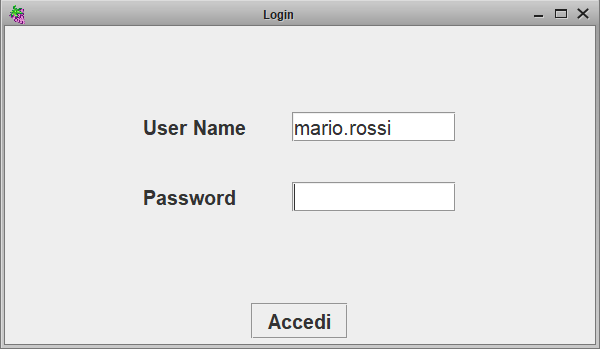
\includegraphics[width=0.7\textwidth]{img/rec_system.png}
\end{figure}\\\newline\newline
\item   \textit{è nel sistema ma non ha effettuato nessun login}, allora deve registarsi, ovvero deve immettere la password e confermarla, e poi può accedere.
\begin{figure}[htbp]
\centering
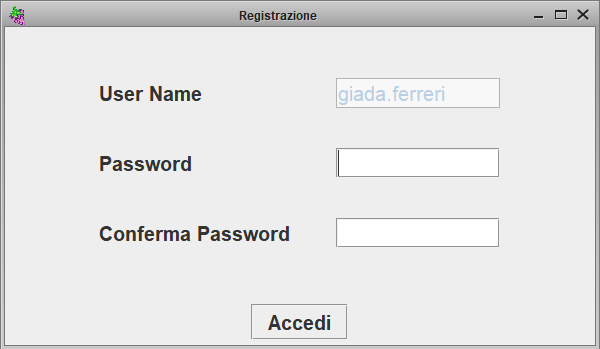
\includegraphics[width=0.7\textwidth]{img/rec_passw.png}
\end{figure}\\\newline\newline
\end{itemize}
\newpage
Dopo essersi loggati, a seconda del ruolo che riveste ciascuna persona (proprietario/amministratore, operaio dipendente o operaio part-time), si hanno differenti interfaccie.\\
\begin{itemize}
\item  \textit{Admin}.\\
Una volta effettuato l'accesso, l'applicativo offre all'amministratore le seguenti possibilità:
\begin{itemize}
\item  \textit{Assumere operai}.
\item  \textit{Registrare le varie fasi e i relativi prodotti}.
\item  \textit{Gestire le vendite e la registrazione dei clienti}.
\item  \textit{Registare gli strumenti dell'azienda (Uva, Botti, Vendemmiatrice)}.
\item  \textit{Effettuare ricerche}.
\end{itemize}
\begin{figure}[htbp]
\centering
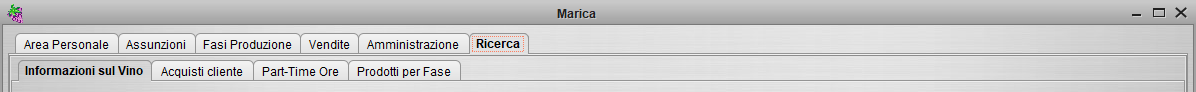
\includegraphics[width=1\textwidth]{img/Panelli_Ricerca_Admin.png}
\end{figure}
\item  \textit{Operaio Dipendente}.\\
Una volta effettuato l'accesso, l'applicativo offre al dipendente le seguenti possibilità:
\begin{itemize}
\item  \textit{Registrare le varie fasi e i relativi prodotti}.
\item  \textit{Gestire le vendite e la registrazione dei clienti}.
\item  \textit{Effettuare ricerche}.
\end{itemize}
\begin{figure}[htbp]
\centering
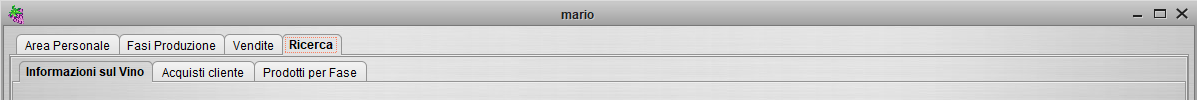
\includegraphics[width=1\textwidth]{img/Panelli_Ricerca_Dip.png}
\end{figure}
\item  \textit{Operaio Part-Time}.\\
Una volta effettuato l'accesso, l'applicativo offre al dipendente part-time le seguenti possibilità:
\begin{itemize}
\item  \textit{Registrare le varie fasi e i relativi prodotti}.
\item  \textit{Effettuare ricerche}.
\end{itemize}
\begin{figure}[htbp]
\centering
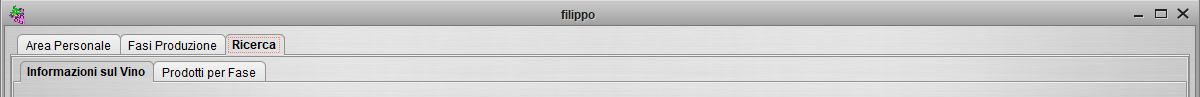
\includegraphics[width=1\textwidth]{img/Panelli_Ricerca_Part.png}
\end{figure}
\end{itemize}
\newpage
\subsection{Descrizione dei pannelli dell'applicazione}
La interfaccia è molto intuitiva, quindi spiegherò brevemente le funzioni dei vari pulsanti.
\subsubsection{Pannello di Assunzione}
\begin{figure}[htbp]
\centering
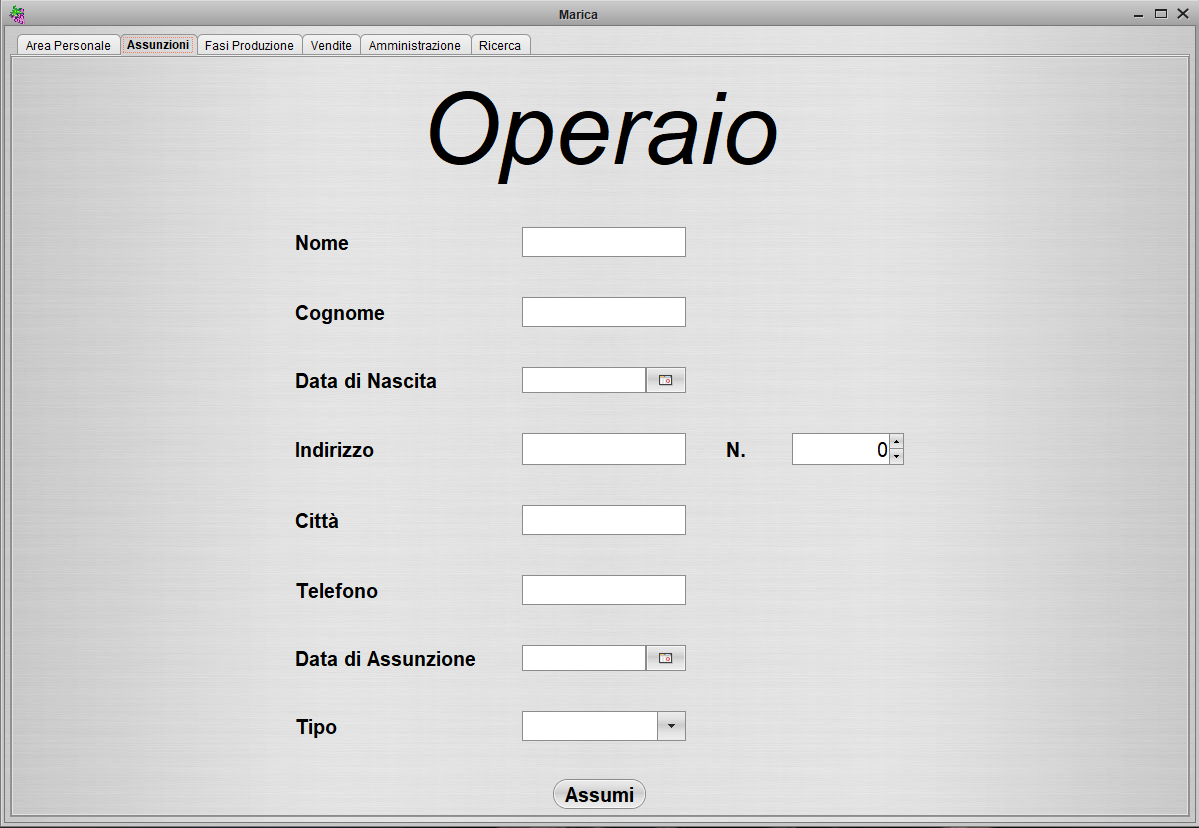
\includegraphics[width=0.6\textwidth]{img/panel_assunzioni.png}
\end{figure}
Il pulsante "Assumi" inserisce un operaio nel database. Nel caso uno o più campi non siano stati compilati viene segnalato.
\subsubsection{Pannello delle Fasi di Produzioni}
\begin{itemize}
\item \textit{Fase}\\
\begin{figure}[htbp]
\centering
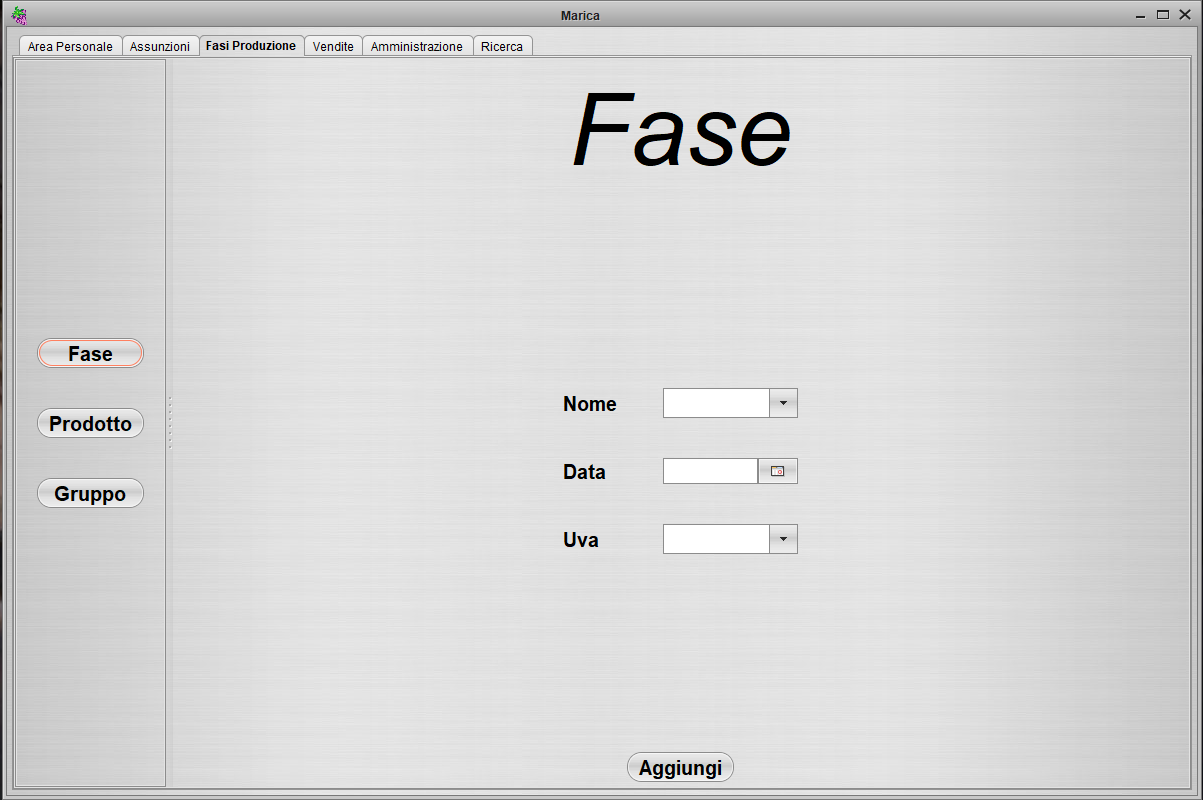
\includegraphics[width=0.7\textwidth]{img/panel_phase.png}
\end{figure}\\
Il pulsante "Aggiungi" inserisce nella tabella (del database) corrispondente a una fase di produzione i vari dati (data e varietà di uva). Nella fase della \textit{Raccolta} verrà richiesto di inserire la quantità di uva raccolta.\\
\newpage
\item \textit{Prodotto}\\
\begin{figure}[htbp]
\centering
\includegraphics[width=0.8\textwidth]{img/panel_product.png}
\end{figure}\\
Il pulsante "Avanti" verifica che la tupla corrispondente agli elementi inseriti nella form (Fase e Uva) esistono nel database. Se non esiste viene segnalato, altrimenti se il prodotto non è già stato inserito, vengono aggiunti i campi necessari a completare l'inserimento del prodotto (figura successiva).
\begin{figure}[htbp]
\centering
\includegraphics[width=0.8\textwidth]{img/panel_product_quantity.png}
\end{figure}\\
Il pulsante "Aggiungi" inserisce nella tabella (del database) corrispondente a un prodotto i vari dati. \\
Il pulsante "Annulla" resetta i vari campi e impedisce l'inserimento del prodotto nel database. \\
\newpage
\item \textit{Gruppo}\\
\begin{figure}[htbp]
\centering
\includegraphics[width=0.8\textwidth]{img/panel_group_init.png}
\end{figure}\\
Il pulsante "Avanti" verifica che la fase selezionata sia inserita. In caso positivo compaiono, nella ComboBox, le date corrispondenti della fase per permettere l'inserimento degli operai (figura successiva).
\begin{figure}[htbp]
\centering
\includegraphics[width=0.8\textwidth]{img/panel_group.png}
\end{figure}\\
Il pulsante "Aggiungi" aggiunge in una lista e nella Table, le informazioni da inserire nel database.\\
Il pulsante "Reset"  resetta i vari campi e impedisce l'inserimento del gruppo nel database.\\
Il pulsante "Chiudi" inserisce nel database l'intera lista.\\
\end{itemize}
\newpage
\subsubsection{Pannello delle Vendite}
\begin{figure}[htbp]
\centering
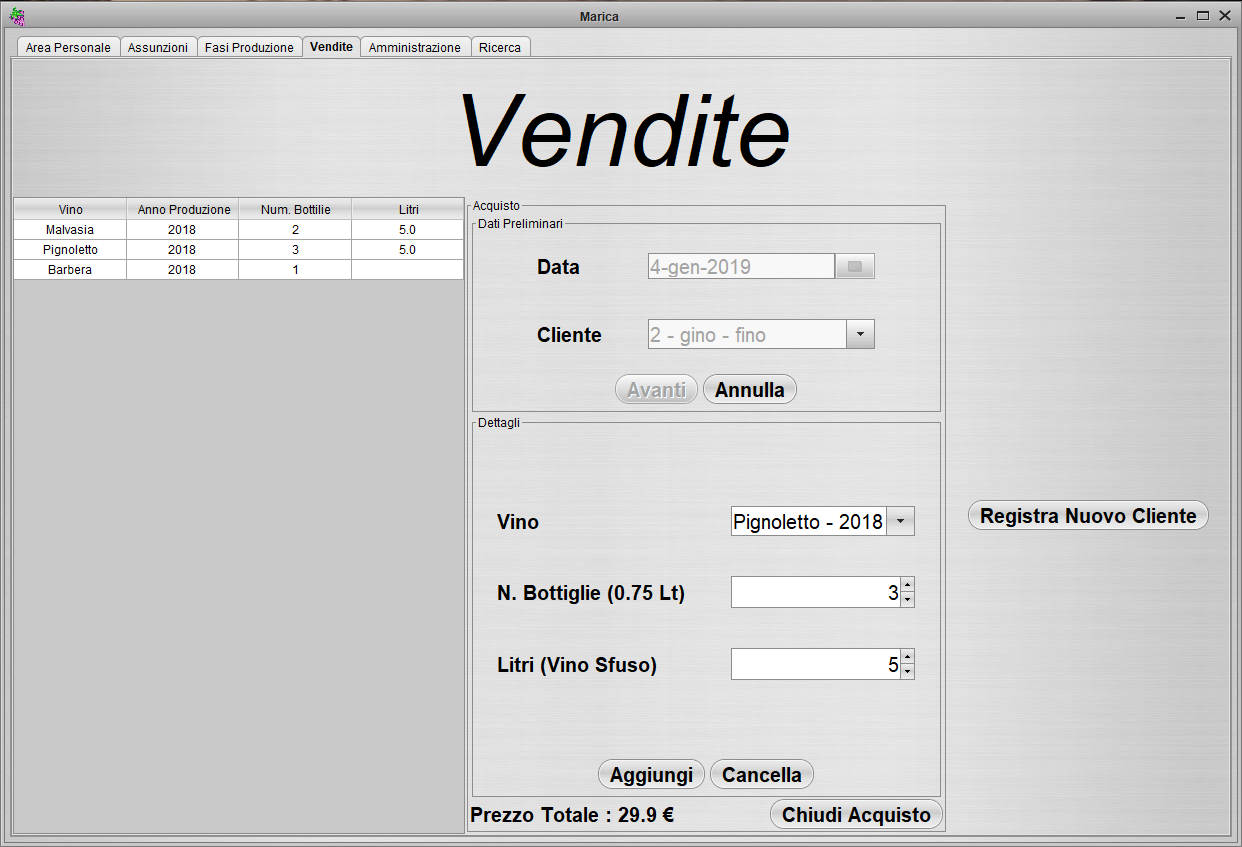
\includegraphics[width=0.8\textwidth]{img/panel_vendite.png}
\end{figure}
Il pulsante "Avanti" memorizza la data di acquisto e l'id del cliente e visualizza il pannello per l'inserimento dei vini nel carrello.\\
Il pulsante "Annulla" annulla l'acquisto e resetta l'interfaccia.\\
Il pulsante "Aggiungi" memorizza nel carrello la quantità di vino selezionato e la inserisce nella Table.\\
Il pulsante "Cancella" rimuove dal carrello, se presente,  il vino selezionato.\\
Il pulsante "Chiudi Acquisto" inserisce nel database l'acquisto e i suoi dettagli.\\
\newline
Nel caso il cliente non sia stato registrato lo si può inserire attraverso il pulsante "Registra Nuovo Cliente" (figura successiva).\\
\begin{figure}[htbp]
\centering
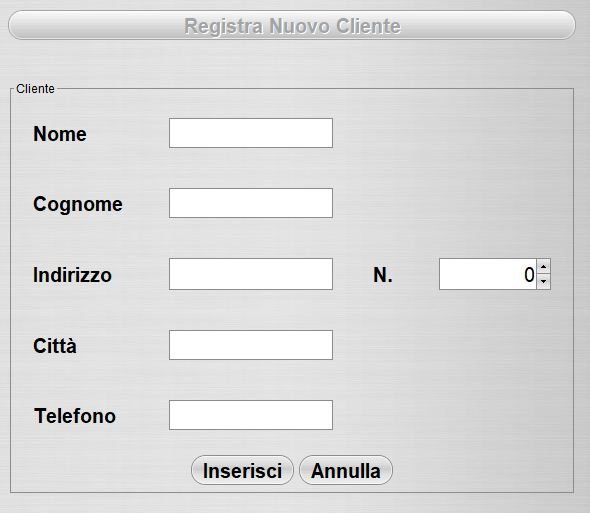
\includegraphics[width=0.5\textwidth]{img/panel_client.png}
\end{figure}\\
Il pulsante "Inserisci" inserisce nel database il cliente e lo inserisce nella ComboBox del pannello Dati Preliminari dell'aquisto.\\
Il pulsante "Annulla" resetta l'interfaccia evitando l'inserimento del cliente.\\
\newpage
\subsubsection{Pannello di Amministrazione}
I pulsanti "Aggiungi ..." mostano i panelli dei vari elementi da inserire.\\
\begin{figure}[htbp]
\centering
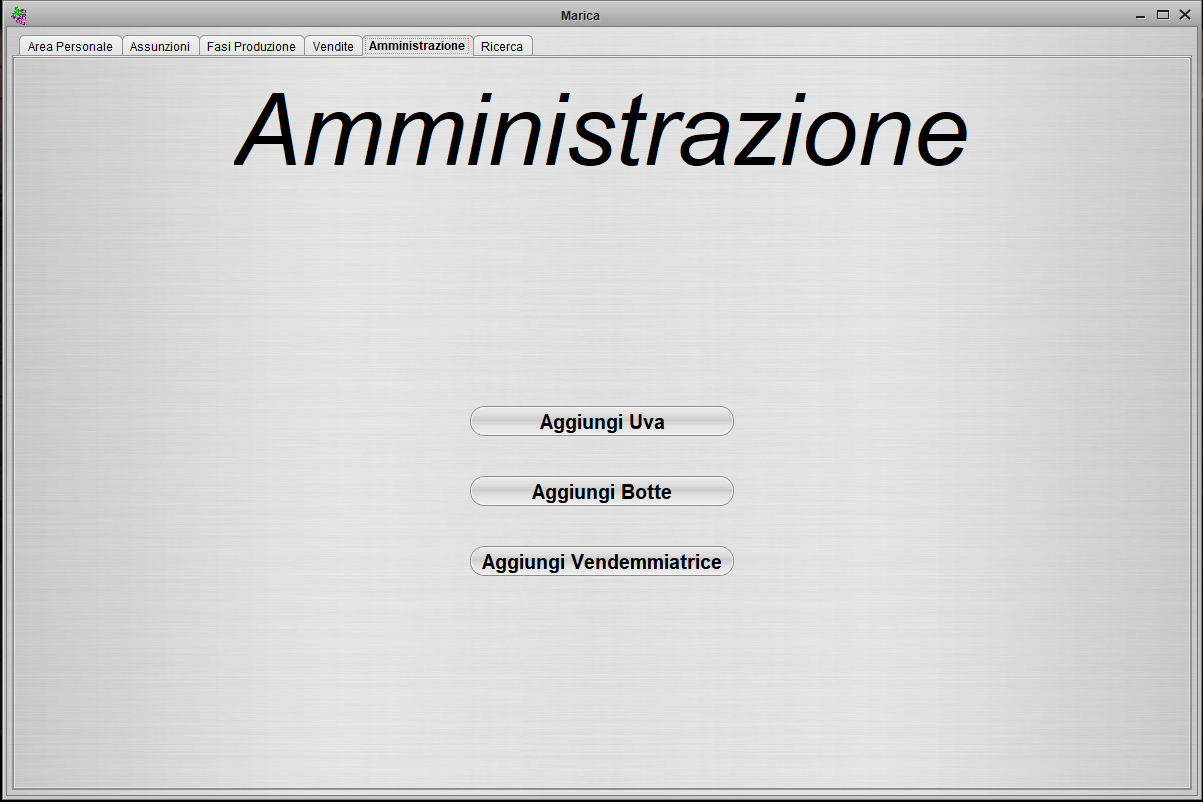
\includegraphics[width=0.7\textwidth]{img/panel_amministrazione_init.png}
\end{figure}\\
\begin{itemize}
\item "Aggiungi Uva " (Varietà del Vitigno):\\
\begin{figure}[htbp]
\centering
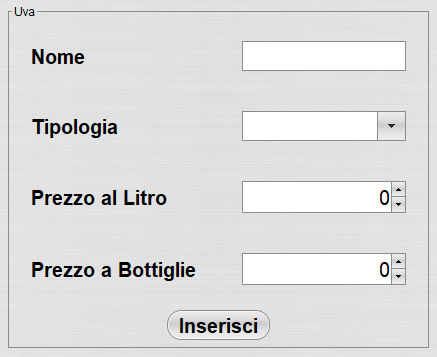
\includegraphics[width=0.5\textwidth]{img/panel_uva.png}
\end{figure}
\newpage
\item "Aggiungi Botte " :\\
\begin{figure}[htbp]
\centering
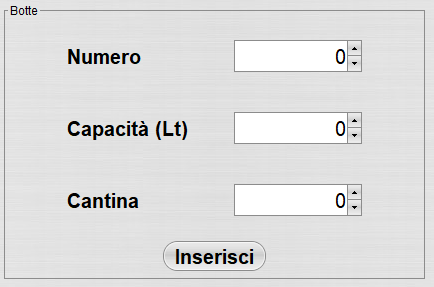
\includegraphics[width=0.5\textwidth]{img/panel_botte.png}
\end{figure}
\item "Aggiungi Vendemmiatrice " :\\
\begin{figure}[htbp]
\centering
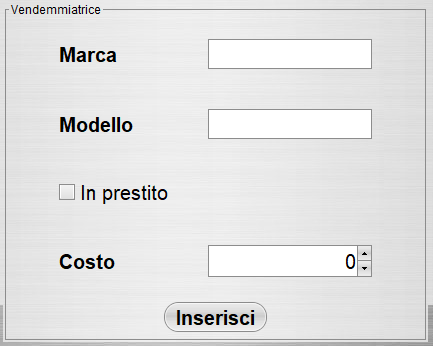
\includegraphics[width=0.5\textwidth]{img/panel_vendemmiatrice.png}
\end{figure}
\end{itemize}
I pulsanti "Inserisci" inseriscono nel database le varie informazioni nelle rispettive tabelle (Uva, Botte, Vendemmiatrice).\\
\newpage
\subsubsection{Panello di Ricerca}
I pulsanti "Ricerca"  eseguono la query ad essa assogiata e visualizza il risultato nella Table.\\
\begin{itemize}
\item Informazioni su un vino \\
La query associata è operazione N. 10.\\
\begin{figure}[htbp]
\centering
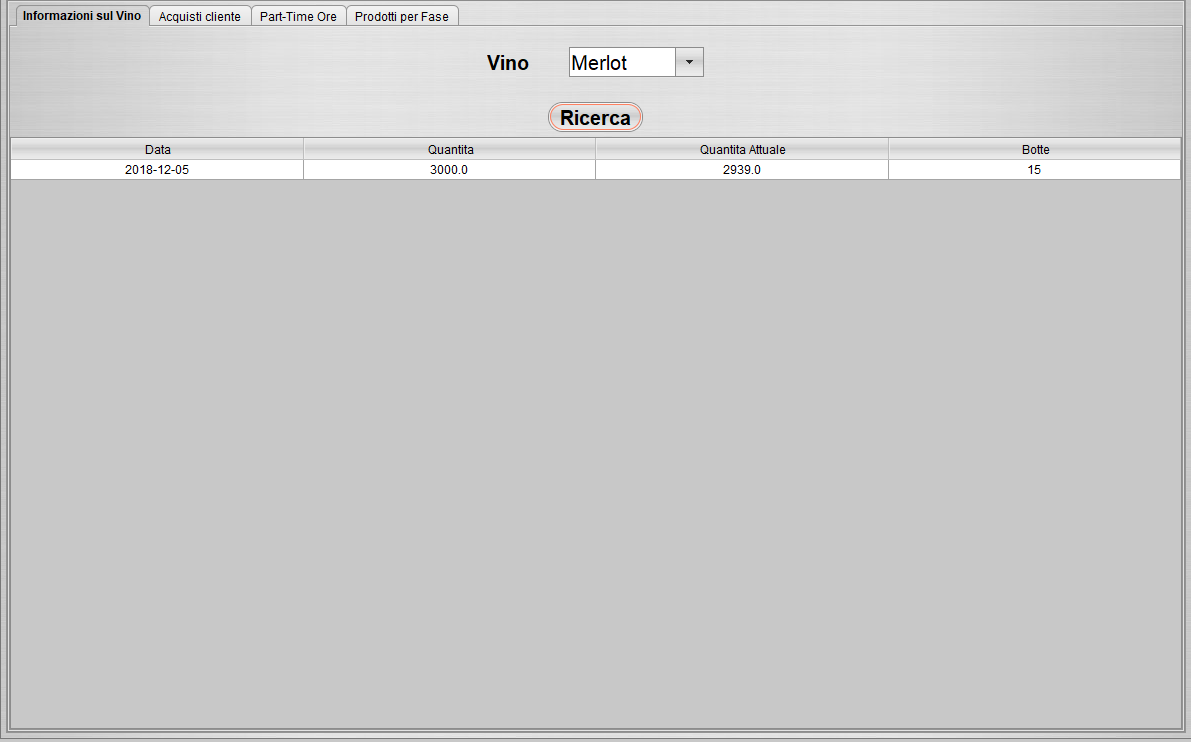
\includegraphics[width=0.8\textwidth]{img/panel_info_vino.png}
\end{figure}
\item Informazioni sull' acqusito di un cliente\\
La query associata è operazione N. 13.\\
\begin{figure}[htbp]
\centering
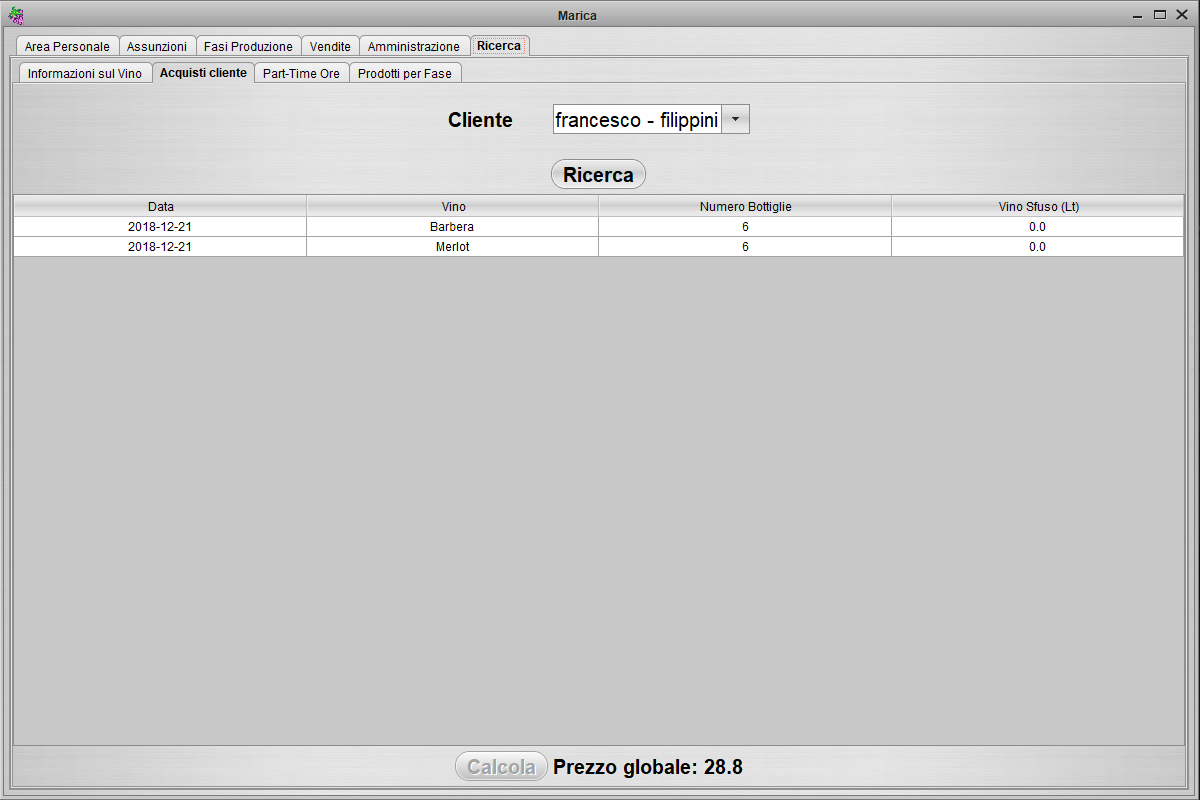
\includegraphics[width=0.8\textwidth]{img/panel_acquisto_cliente.png}
\end{figure}\newline
Il pulsante "Calcola" calcola la somma di tutti i vini acquistati da tale cliente.\\
\newpage
\item Informazioni su ore di lavoro di un operaio part-time\\
La query associata è operazione N. 12.\\
\begin{figure}[htbp]
\centering
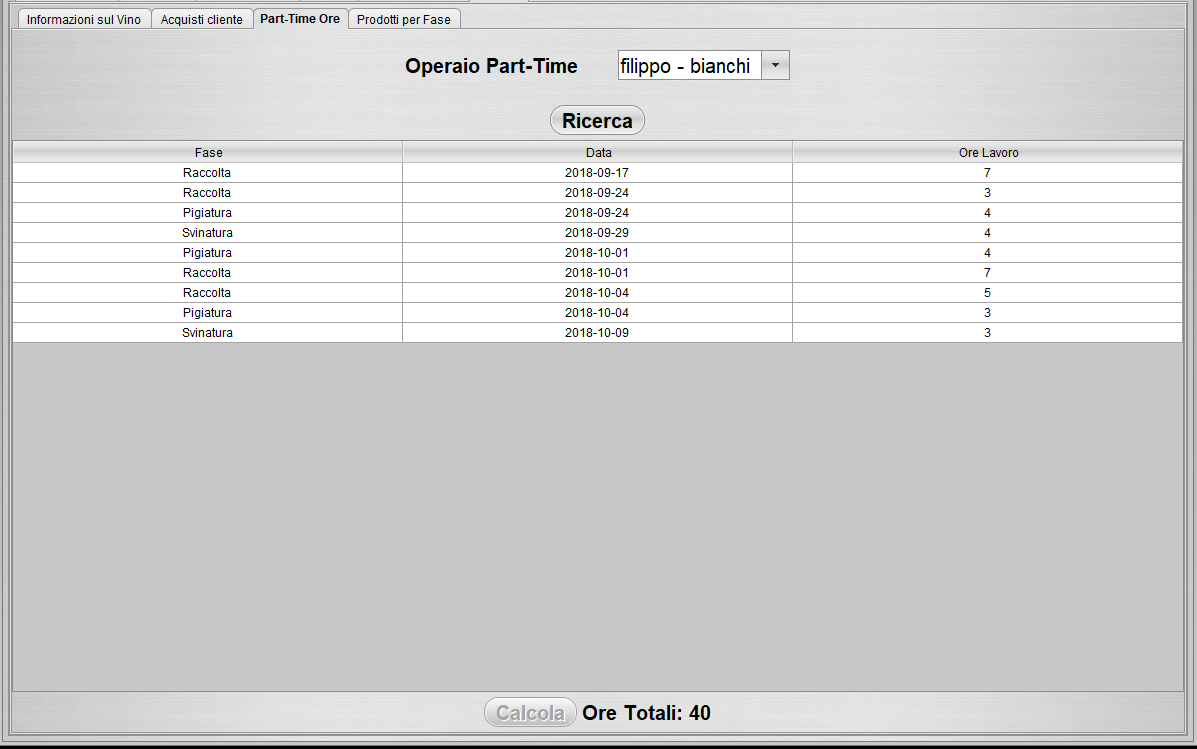
\includegraphics[width=0.8\textwidth]{img/panel_part_ore.png}
\end{figure}\newline
Il pulsante "Calcola" calcola la somma di tutte le Ore di Lavoro.\\
\item Informazioni sui prodotti di una fase di un dato anno \\
La query associata è operazione N. 11.\\
\begin{figure}[htbp]
\centering
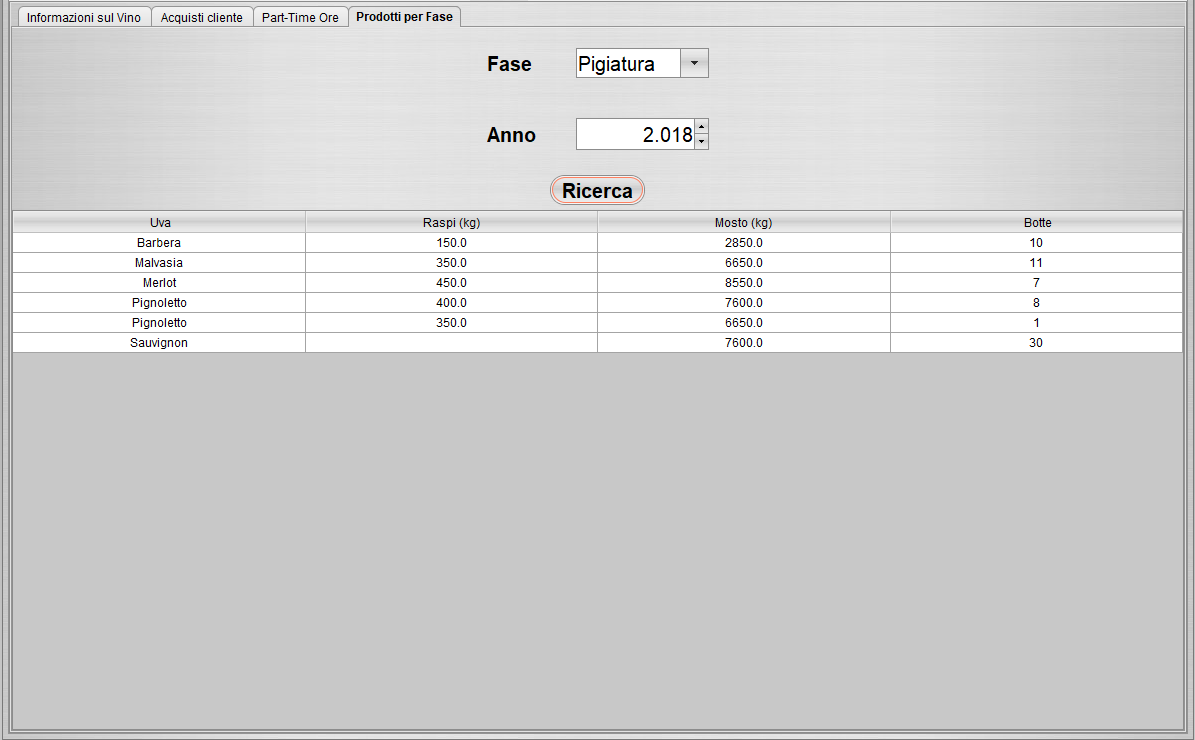
\includegraphics[width=0.8\textwidth]{img/panel_info_prodotti.png}
\end{figure}
\end{itemize}

\end{document}
